\documentclass[aspectratio=169,12pt,t]{beamer}

% --- Theme: Metropolis (modern, clean) ---
\usetheme[progressbar=frametitle,numbering=fraction,block=fill]{metropolis}

% --- Fira Sans font (install texlive-fonts-extra if missing) ---
\IfFileExists{FiraSans.sty}{\usepackage[sfdefault]{FiraSans}}{}

% --- Light background with warm accent ---
\definecolor{mDarkTeal}{RGB}{35,55,59}
\definecolor{mLightBrown}{RGB}{235,228,216}
\definecolor{mAccent}{RGB}{140,70,20}

\setbeamercolor{normal text}{fg=mDarkTeal,bg=white}
\setbeamercolor{alerted text}{fg=mAccent}
\setbeamercolor{frametitle}{bg=mDarkTeal,fg=white}
\setbeamercolor{progress bar}{fg=mAccent,bg=mLightBrown}
\setbeamercolor{title separator}{fg=mAccent}
\setbeamercolor{progress bar in head/foot}{fg=mAccent,bg=mLightBrown}
\setbeamercolor{progress bar in section page}{fg=mAccent,bg=mLightBrown}

% --- Packages ---
\usepackage[utf8]{inputenc}
\usepackage{amsmath,amssymb,amsthm}
\usepackage{mathrsfs}
\usepackage{tikz}
\usetikzlibrary{arrows.meta,positioning,calc,decorations.pathreplacing,shapes,patterns,backgrounds}
\usepackage{pgfplots}
\pgfplotsset{compat=1.18}
\usepgfplotslibrary{fillbetween}

% --- TikZ diagram styles (shared across the series) ---
\tikzset{
  bgveil/.style={show background rectangle, inner frame sep=4pt,
    background rectangle/.style={fill=white, fill opacity=0.6, draw=none}},
  axisln/.style={-{Stealth[length=2.6mm]}, line width=0.8pt, gray!75},
  curveln/.style={line width=1.6pt, line cap=round, line join=round},
  projln/.style={dash pattern=on 2.6pt off 2pt, line width=0.7pt},
  guide/.style={-{Stealth[length=2.6mm,width=2.2mm]}, line width=1.1pt},
  box/.style={draw=#1, fill=#1!12, line width=1pt, rounded corners=2pt,
    minimum width=5.6cm, minimum height=1.35cm, align=center, font=\small},
}
% point marker with a white halo: \dotpt{color}{(coord)}
\newcommand{\dotpt}[2]{%
  \fill[white] #2 circle (3.6pt);
  \fill[#1] #2 circle (2.4pt);
}
% open point marker: \opendotpt{color}{(coord)}
\newcommand{\opendotpt}[2]{%
  \fill[white] #2 circle (3.6pt);
  \draw[#1, line width=1pt] #2 circle (2.4pt);
}

% --- Semi-transparent white highlight for text on top of background images ---
\usepackage[most]{tcolorbox}

% Inline highlight: \hl{short text}
\newtcbox{\hl}{%
  nobeforeafter, tcbox raise base,
  colback=white, opacityback=0.6,
  colframe=white, opacityframe=0,
  sharp corners, boxsep=2pt, left=3pt, right=3pt, top=2pt, bottom=2pt%
}

% Block highlight: \begin{hlbox} ... \end{hlbox}  (multi-line, paragraphs, itemize)
% Optional argument accepts any tcolorbox key, e.g. [width=0.6\linewidth]
\newtcolorbox{hlbox}[1][]{%
  enhanced, breakable,
  colback=white, opacityback=0.6,
  colframe=white, opacityframe=0,
  boxsep=3pt, left=6pt, right=6pt, top=4pt, bottom=4pt,
  sharp corners,
  {#1}%
}

% --- Custom colors for content types ---
\definecolor{defcolor}{RGB}{25,85,120}
\definecolor{thmcolor}{RGB}{140,35,35}
\definecolor{proofcolor}{RGB}{35,100,50}
\definecolor{excolor}{RGB}{140,75,10}
\definecolor{remcolor}{RGB}{90,90,90}

% --- Beamer blocks for mathematical content types (semi-transparent) ---
\tcbset{hlblockbase/.style={
  enhanced, breakable,
  coltitle=white, fonttitle=\bfseries,
  opacitybacktitle=0.8, opacityback=0.6,
  opacityframe=0,
  sharp corners,
  boxsep=1pt, left=5pt, right=5pt, top=2pt, bottom=2pt,
  toptitle=1pt, bottomtitle=1pt,
  before upper={\setlength{\abovedisplayskip}{4pt}\setlength{\belowdisplayskip}{4pt}}
}}

\newtcolorbox{defblock}[1]{hlblockbase, title={#1},
  colbacktitle=defcolor, colback=defcolor!15, colframe=defcolor}
\newtcolorbox{thmblock}[1]{hlblockbase, title={#1},
  colbacktitle=thmcolor, colback=thmcolor!15, colframe=thmcolor}
\newtcolorbox{proofblock}[1]{hlblockbase, title={#1},
  colbacktitle=proofcolor, colback=proofcolor!15, colframe=proofcolor}
\newtcolorbox{exblock}[1]{hlblockbase, title={#1},
  colbacktitle=excolor, colback=excolor!15, colframe=excolor}
\newtcolorbox{remblock}[1]{hlblockbase, title={#1},
  colbacktitle=remcolor, colback=remcolor!15, colframe=remcolor}


% --- Metadata ---
\title{Chapter 7: Sequences and Series of Functions}
\subtitle{Section: Uniform Convergence and Differentiation}
\author{Based on Walter Rudin's \emph{Principles of Mathematical Analysis}}
\date{}

% --- Shared plot helpers for this deck ---
% Sawtooth of Theorem 7.18: phi(x) = |x| on [-1,1], period 2
\pgfmathdeclarefunction{saw}{1}{\pgfmathparse{abs((#1) - 2*floor(((#1)+1)/2))}}

\begin{document}

{
\usebackgroundtemplate{%
  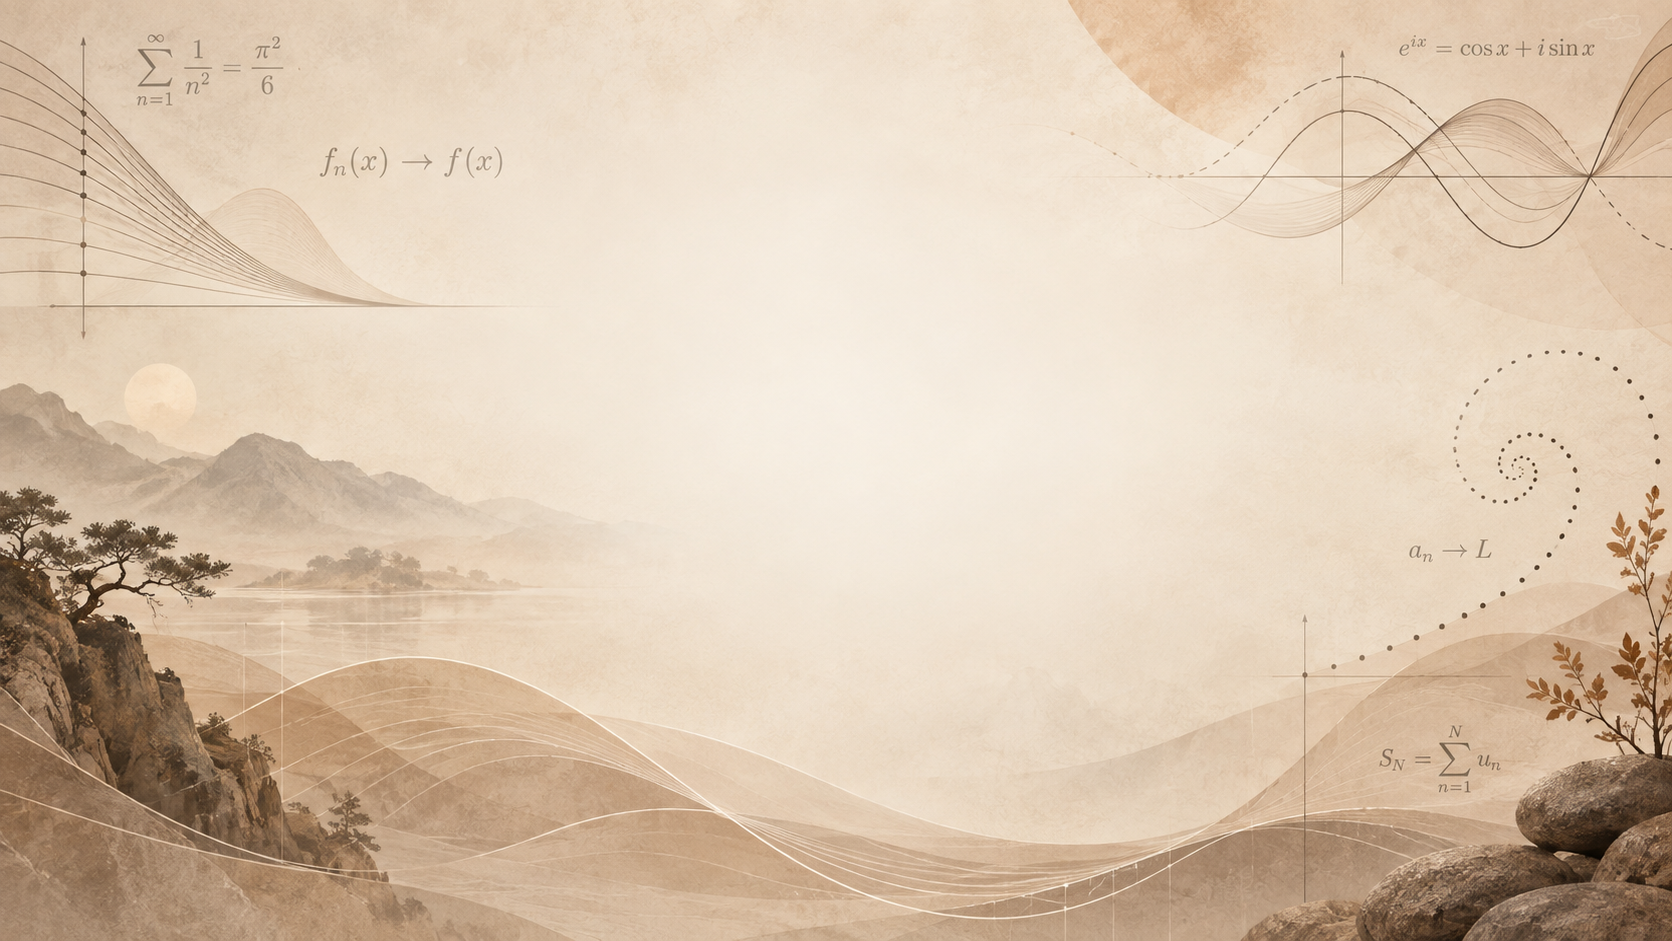
\includegraphics[width=\paperwidth,height=\paperheight,keepaspectratio=false]{chapter_07_bg_00.png}%
}
\begin{frame}[plain]
  \titlepage

  \note{
    Welcome back to Chapter 7, Sequences and Series of Functions. This
    is the fifth section, Uniform Convergence and Differentiation. So
    far we have seen that uniform convergence preserves continuity and
    integrals. Derivatives are a different story. In this section we
    find the right hypothesis under which the derivative of the limit
    is the limit of the derivatives. Then we meet one of the most
    surprising objects in analysis: a continuous function on the real
    line that has no derivative at any point. Let's begin.
  }
\end{frame}
}

{
\usebackgroundtemplate{%
  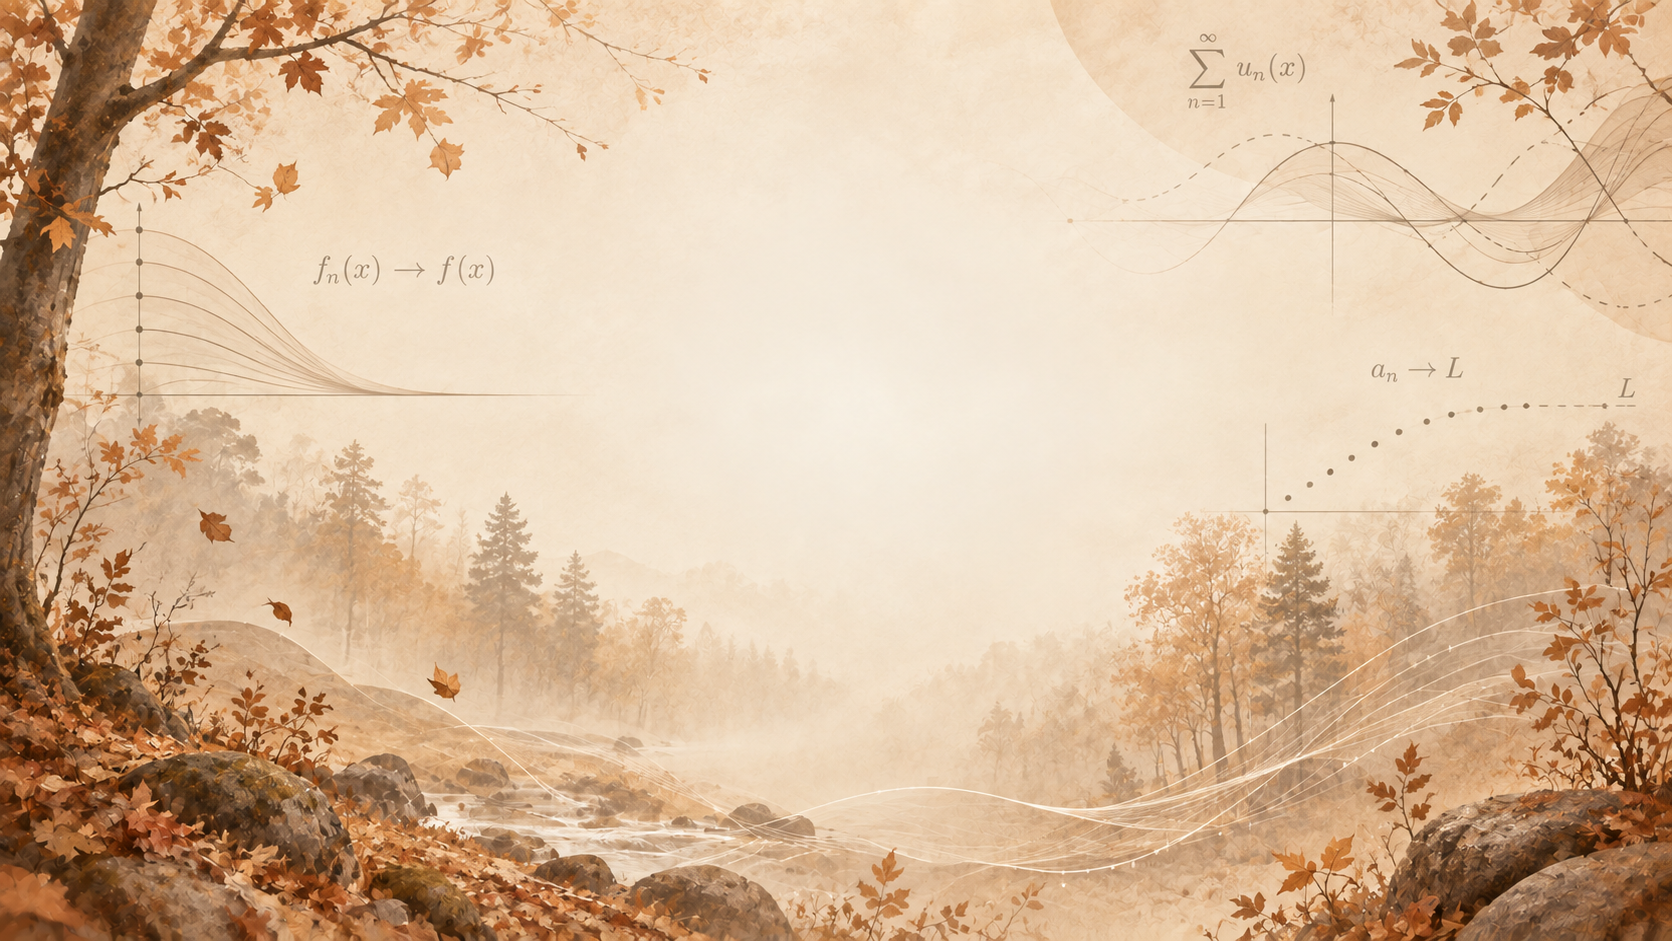
\includegraphics[width=\paperwidth,height=\paperheight,keepaspectratio=false]{chapter_07_bg_01.png}%
}
\begin{frame}[c]{Outline}
  \begin{center}
    \tableofcontents
  \end{center}

  \note{
    Here is the plan. We start with a short motivation, recalling Example
    7.5, which shows that uniform convergence of the functions says
    nothing about their derivatives. The second part, Differentiating a
    Limit, states Theorem 7.17, and the third part proves it. Then comes
    Nowhere Differentiable Function, where we construct the example of
    Theorem 7.18, followed by the proof that it really has no derivative
    anywhere. We close with a summary.
  }
\end{frame}

\section{Motivation}

% --- Build 1/3 ---
\begin{frame}{Why This Section Matters}
  \begin{hlbox}
  \begin{itemize}
    \item The \alert{main problem} of Section 7.1, now for derivatives:
      \[
        \Bigl( \lim_{n \to \infty} f_n \Bigr)'(x)
        \;\overset{?}{=}\;
        \lim_{n \to \infty} f_n'(x)
      \]
  \end{itemize}
  \end{hlbox}

  \note{
    Recall the main problem of this chapter: which properties of the
    functions "f" sub "n" survive the passage to the limit? We have
    handled continuity and integration. The last item on the list is
    differentiation. The question on the slide asks whether we may
    first take the limit of the functions and then differentiate, and
    get the same answer as differentiating each "f" sub "n" first and
    then taking the limit. Both sides involve a limit, since a
    derivative is itself a limit, so this is again a question about
    interchanging two limits.
  }
\end{frame}

% --- Build 2/3 ---
\begin{frame}{Why This Section Matters}
  \begin{hlbox}
  \begin{itemize}
    \item The \alert{main problem} of Section 7.1, now for derivatives:
      \[
        \Bigl( \lim_{n \to \infty} f_n \Bigr)'(x)
        \;\overset{?}{=}\;
        \lim_{n \to \infty} f_n'(x)
      \]
    \item Even \emph{uniform} convergence $f_n \to f$ is \alert{not enough}
      (Example 7.5)
  \end{itemize}
  \end{hlbox}

  \note{
    For integrals, uniform convergence settled the question. For
    derivatives it does not. Example 7.5 gives a sequence that
    converges uniformly to zero, while the derivatives do not converge
    to zero; at the origin they even blow up. The reason is simple: a
    function can be uniformly tiny and still wiggle very fast, and fast
    wiggles mean large slopes. Smallness of values says nothing about
    smallness of slopes.
  }
\end{frame}

% --- Build 3/3 ---
\begin{frame}{Why This Section Matters}
  \begin{hlbox}
  \begin{itemize}
    \item The \alert{main problem} of Section 7.1, now for derivatives:
      \[
        \Bigl( \lim_{n \to \infty} f_n \Bigr)'(x)
        \;\overset{?}{=}\;
        \lim_{n \to \infty} f_n'(x)
      \]
    \item Even \emph{uniform} convergence $f_n \to f$ is \alert{not enough}
      (Example 7.5)
    \item \textbf{Theorem 7.17:} assume instead that the \alert{derivatives}
      $f_n'$ converge uniformly
    \item \textbf{Theorem 7.18:} a uniform limit of continuous functions can be
      \alert{nowhere differentiable}
  \end{itemize}
  \end{hlbox}

  \note{
    This section gives two answers. Theorem 7.17 shows that the right
    hypothesis is uniform convergence of the derivatives, together with
    convergence at just one point. Theorem 7.18 shows how badly things
    can fail otherwise: a uniformly convergent series of very nice
    functions can add up to a continuous function that has no
    derivative at any point at all. Before we start, let's look at
    Example 7.5 once more.
  }
\end{frame}

\begin{frame}{Recall Example 7.5: Small Values, Large Slopes}
  \begin{columns}[T]
    \begin{column}{0.5\textwidth}
      \centering
      \hl{\small $f_n(x) = \dfrac{\sin nx}{\sqrt n} \;\to\; 0$ uniformly}\\[0.2em]
      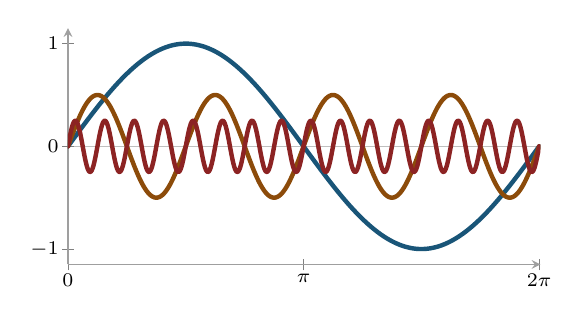
\begin{tikzpicture}
        \begin{axis}[
          axis background/.style={fill=white, fill opacity=0.6},
          scale only axis, width=6.0cm, height=3.0cm,
          xmin=0, xmax=6.3, ymin=-1.15, ymax=1.15,
          axis x line=bottom, axis y line=left, axis line style={gray!75},
          xtick={0,3.1416,6.2832}, xticklabels={$0$,$\pi$,$2\pi$},
          extra y ticks={0}, extra y tick style={grid=major, major grid style={gray!50}},
          ytick={-1,1},
          tick label style={font=\scriptsize, fill=white, fill opacity=0.6, text opacity=1, inner sep=1pt},
          every axis plot/.append style={curveln},
        ]
          \addplot[domain=0:6.2832, samples=200, defcolor] {sin(deg(x))};
          \addplot[domain=0:6.2832, samples=300, excolor] {sin(deg(4*x))/2};
          \addplot[domain=0:6.2832, samples=500, thmcolor] {sin(deg(16*x))/4};
        \end{axis}
      \end{tikzpicture}
    \end{column}
    \begin{column}{0.5\textwidth}
      \centering
      \hl{\small $\vphantom{\dfrac{\sin nx}{\sqrt n}}f_n'(x) = \sqrt n \cos nx$ \alert{does not} converge}\\[0.2em]
      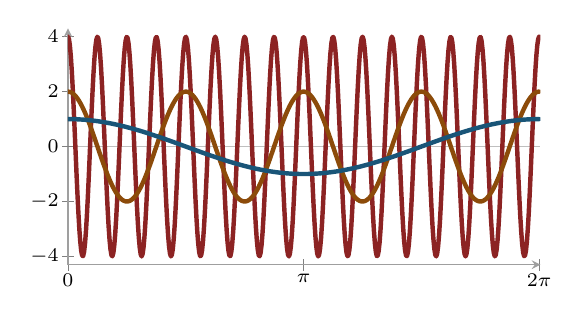
\begin{tikzpicture}
        \begin{axis}[
          axis background/.style={fill=white, fill opacity=0.6},
          scale only axis, width=6.0cm, height=3.0cm,
          xmin=0, xmax=6.3, ymin=-4.3, ymax=4.3,
          axis x line=bottom, axis y line=left, axis line style={gray!75},
          xtick={0,3.1416,6.2832}, xticklabels={$0$,$\pi$,$2\pi$},
          extra y ticks={0}, extra y tick style={grid=major, major grid style={gray!50}},
          ytick={-4,-2,2,4},
          tick label style={font=\scriptsize, fill=white, fill opacity=0.6, text opacity=1, inner sep=1pt},
          every axis plot/.append style={curveln},
        ]
          \addplot[domain=0:6.2832, samples=500, thmcolor] {4*cos(deg(16*x))};
          \addplot[domain=0:6.2832, samples=300, excolor] {2*cos(deg(4*x))};
          \addplot[domain=0:6.2832, samples=200, defcolor] {cos(deg(x))};
        \end{axis}
      \end{tikzpicture}
    \end{column}
  \end{columns}

  \vspace{0.3em}
  \begin{center}
    \hl{\small
    \textcolor{defcolor}{$n=1$} \quad \textcolor{excolor}{$n=4$} \quad
    \textcolor{thmcolor}{$n=16$}
    \qquad
    $f' \equiv 0$, \; but $f_n'(0) = \sqrt n \to +\infty$}
  \end{center}

  \note{
    Here is Example 7.5 again, with both plots drawn from 0 to 2 pi. On
    the left are the functions sine of "n" "x" divided by the square root
    of "n", for "n" equal to 1 in blue, 4 in brown, and 16 in red, as the
    color key at the bottom shows. Their height is one over the square
    root of "n", so they flatten out and converge uniformly to the zero
    function, whose derivative is zero. On the right are their
    derivatives, the square root of "n" times cosine of "n" "x", in the
    same colors. Here the picture is reversed: the waves get faster and
    taller. They do not converge at all, and at the origin they equal the
    square root of "n", which tends to infinity, as the bottom line of the
    slide says. Notice the scales: the left plot goes up to 1, the right
    one up to 4.
  }
\end{frame}

\begin{frame}{Roadmap of This Section}
  \vspace{0.6em}
  \begin{center}
  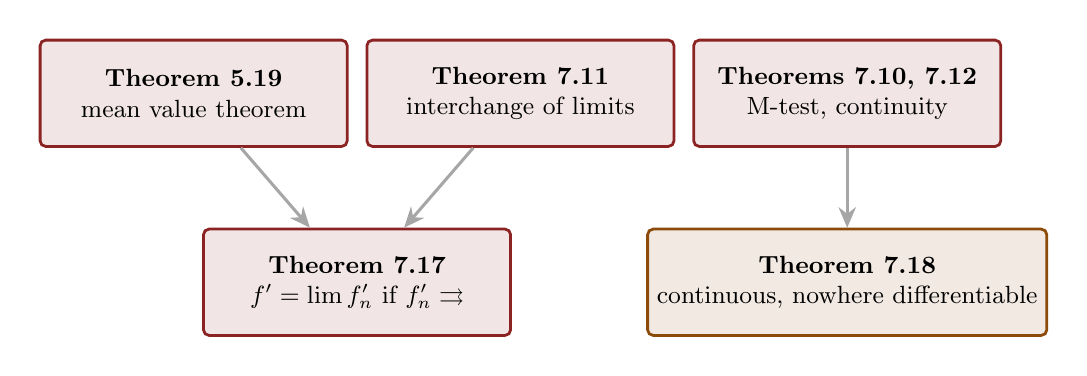
\begin{tikzpicture}[bgveil]
    \node[box=thmcolor, minimum width=3.9cm] (a) at (-4.15,0) {\textbf{Theorem 5.19}\\ mean value theorem};
    \node[box=thmcolor, minimum width=3.9cm] (b) at (0,0) {\textbf{Theorem 7.11}\\ interchange of limits};
    \node[box=thmcolor, minimum width=3.9cm] (e) at (4.15,0) {\textbf{Theorems 7.10, 7.12}\\ M-test, continuity};
    \node[box=thmcolor, minimum width=3.9cm] (c) at (-2.075,-2.4) {\textbf{Theorem 7.17}\\ $f' = \lim f_n'$ if $f_n' \rightrightarrows$};
    \node[box=excolor, minimum width=3.9cm] (d) at (4.15,-2.4) {\textbf{Theorem 7.18}\\ continuous, nowhere differentiable};
    \draw[guide, gray!70] (a) -- (c);
    \draw[guide, gray!70] (b) -- (c);
    \draw[guide, gray!70] (e) -- (d);
  \end{tikzpicture}
  \end{center}

  \note{
    The diagram shows the structure. In the top row are two tools we
    already have: the mean value theorem, Theorem 5.19, on the left,
    Theorem 7.11 on interchanging limits, in the middle, and the M-test
    and continuity theorems on the right. Gray arrows lead from the
    first two down to Theorem 7.17, which says that the
    derivative of the limit is the limit of the derivatives when the
    derivatives converge uniformly; the double arrow symbol is a common
    shorthand for uniform convergence. On the right, the M-test and the
    continuity theorem lead down to Theorem 7.18 in brown, the nowhere
    differentiable function.
  }
\end{frame}
}

{
\usebackgroundtemplate{%
  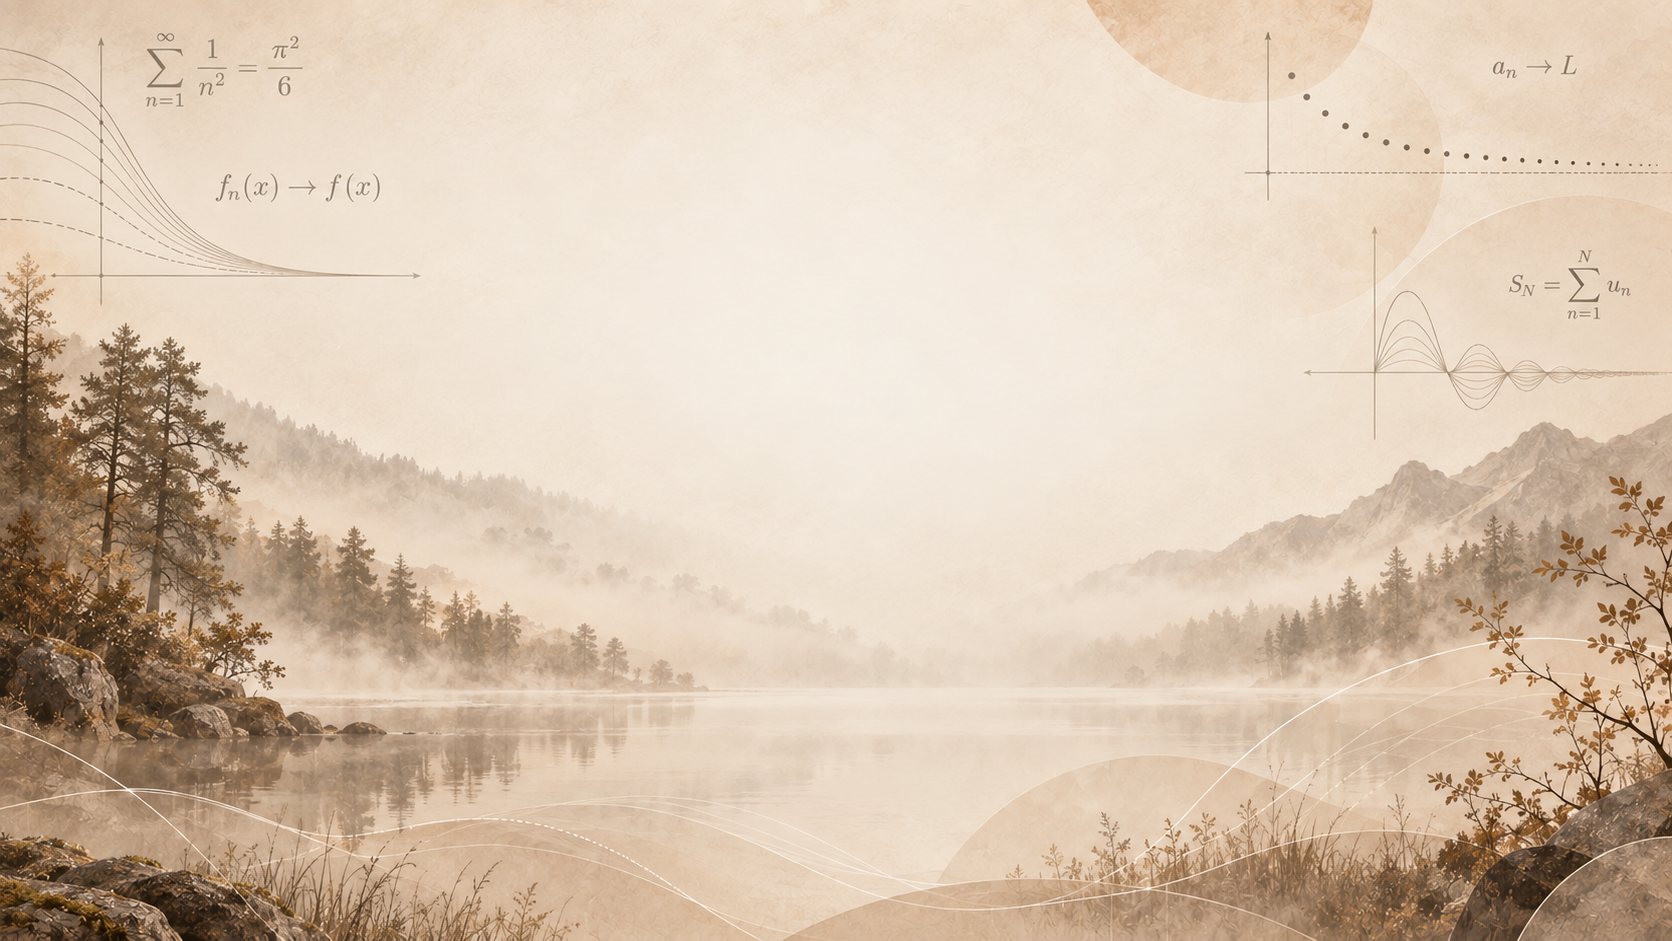
\includegraphics[width=\paperwidth,height=\paperheight,keepaspectratio=false]{chapter_07_bg_02.png}%
}
\section{Differentiating a Limit}

% --- Build 1/2 ---
\begin{frame}{Theorem 7.17: Differentiating a Limit}
  \begin{thmblock}{Theorem 7.17}
    Suppose $\{f_n\}$ is a sequence of functions, differentiable on $[a, b]$
    and such that $\{f_n(x_0)\}$ converges for \alert{some point} $x_0$ on
    $[a, b]$. If $\{f'_n\}$ converges \alert{uniformly} on $[a, b]$, then
    $\{f_n\}$ converges uniformly on $[a, b]$, to a function $f$, and
    \begin{equation}
      f'(x) = \lim_{n \to \infty} f'_n(x) \qquad (a \leq x \leq b). \tag{27}
    \end{equation}
  \end{thmblock}

  \note{
    Here is Theorem 7.17. Each "f" sub "n" is differentiable on the
    closed interval from "a" to "b". We assume two things. First, at a
    single point "x" sub zero, the numbers "f" sub "n" of "x" sub zero
    converge. Second, the derivatives converge uniformly on the whole
    interval. The conclusion is that the functions themselves converge
    uniformly to some limit "f", and equation 27 holds: "f" is
    differentiable, and its derivative at every point is the limit of
    the derivatives of "f" sub "n".
  }
\end{frame}

% --- Build 2/2 ---
\begin{frame}{Theorem 7.17: Differentiating a Limit}
  \begin{thmblock}{Theorem 7.17}
    Suppose $\{f_n\}$ is a sequence of functions, differentiable on $[a, b]$
    and such that $\{f_n(x_0)\}$ converges for \alert{some point} $x_0$ on
    $[a, b]$. If $\{f'_n\}$ converges \alert{uniformly} on $[a, b]$, then
    $\{f_n\}$ converges uniformly on $[a, b]$, to a function $f$, and
    \begin{equation}
      f'(x) = \lim_{n \to \infty} f'_n(x) \qquad (a \leq x \leq b). \tag{27}
    \end{equation}
  \end{thmblock}
  \begin{remblock}{In words}
    \[
      \Bigl( \lim_{n \to \infty} f_n \Bigr)' = \lim_{n \to \infty} f_n'
      \qquad \text{\small(differentiation and limit \alert{commute})}
    \]
  \end{remblock}

  \note{
    The gray box restates the conclusion in the form of the main
    problem: the derivative of the limit equals the limit of the
    derivatives, so differentiation and the limit commute. Notice how
    the hypotheses are arranged. The uniform convergence is placed on
    the derivatives, not on the functions. Uniform convergence of the
    functions then comes out as part of the conclusion. Let's see why
    each hypothesis is there.
  }
\end{frame}

% --- Build 1/3 ---
\begin{frame}{The Role of Each Hypothesis}
  \begin{hlbox}
  \begin{itemize}
    \item \textbf{Why $f_n'$ and not $f_n$?}\\
      Example 7.5: $f_n \to 0$ uniformly, but $f_n'$ diverges.
      Control of \emph{slopes} needs a hypothesis on \emph{slopes}.
  \end{itemize}
  \end{hlbox}

  \note{
    First, why must the hypothesis be about the derivatives? Example
    7.5 already answered this. Uniform convergence of the functions
    controls their values, but derivatives measure slopes, and values
    can be uniformly small while slopes are huge. To conclude something
    about slopes of the limit, we must assume something about the
    slopes of "f" sub "n".
  }
\end{frame}

% --- Build 2/3 ---
\begin{frame}{The Role of Each Hypothesis}
  \begin{hlbox}
  \begin{itemize}
    \item \textbf{Why $f_n'$ and not $f_n$?}\\
      Example 7.5: $f_n \to 0$ uniformly, but $f_n'$ diverges.
      Control of \emph{slopes} needs a hypothesis on \emph{slopes}.
    \item \textbf{Why convergence at a point $x_0$?}\\
      $f_n(x) = n$: \; $f_n' = 0$ converges uniformly, but $f_n$ diverges.
  \end{itemize}
  \end{hlbox}

  \note{
    Second, why do we need convergence at one point "x" sub zero? Take
    the constant functions "f" sub "n" equal to "n". All derivatives
    are zero, so they certainly converge uniformly, yet the functions
    run off to infinity. Knowing the derivatives determines a function
    only up to an additive constant. Convergence at "x" sub zero pins
    down that constant, like an initial condition in a differential
    equation.
  }
\end{frame}

% --- Build 3/3 ---
\begin{frame}{The Role of Each Hypothesis}
  \begin{hlbox}
  \begin{itemize}
    \item \textbf{Why $f_n'$ and not $f_n$?}\\
      Example 7.5: $f_n \to 0$ uniformly, but $f_n'$ diverges.
      Control of \emph{slopes} needs a hypothesis on \emph{slopes}.
    \item \textbf{Why convergence at a point $x_0$?}\\
      $f_n(x) = n$: \; $f_n' = 0$ converges uniformly, but $f_n$ diverges.
    \item \textbf{Why is one point enough?}\\
      Slopes control \emph{changes}: values at $x_0$ $+$ uniform slopes
      $\Rightarrow$ values everywhere.
  \end{itemize}
  \end{hlbox}

  \note{
    And why is a single point enough? Because the derivatives control
    how much a function can change between two points. If the values
    at "x" sub zero settle down, and the slopes settle down uniformly,
    then the values at every other point must settle down too. This is
    exactly the first part of the proof, which uses the mean value
    theorem. Let's turn to the proof.
  }
\end{frame}
}

{
\usebackgroundtemplate{%
  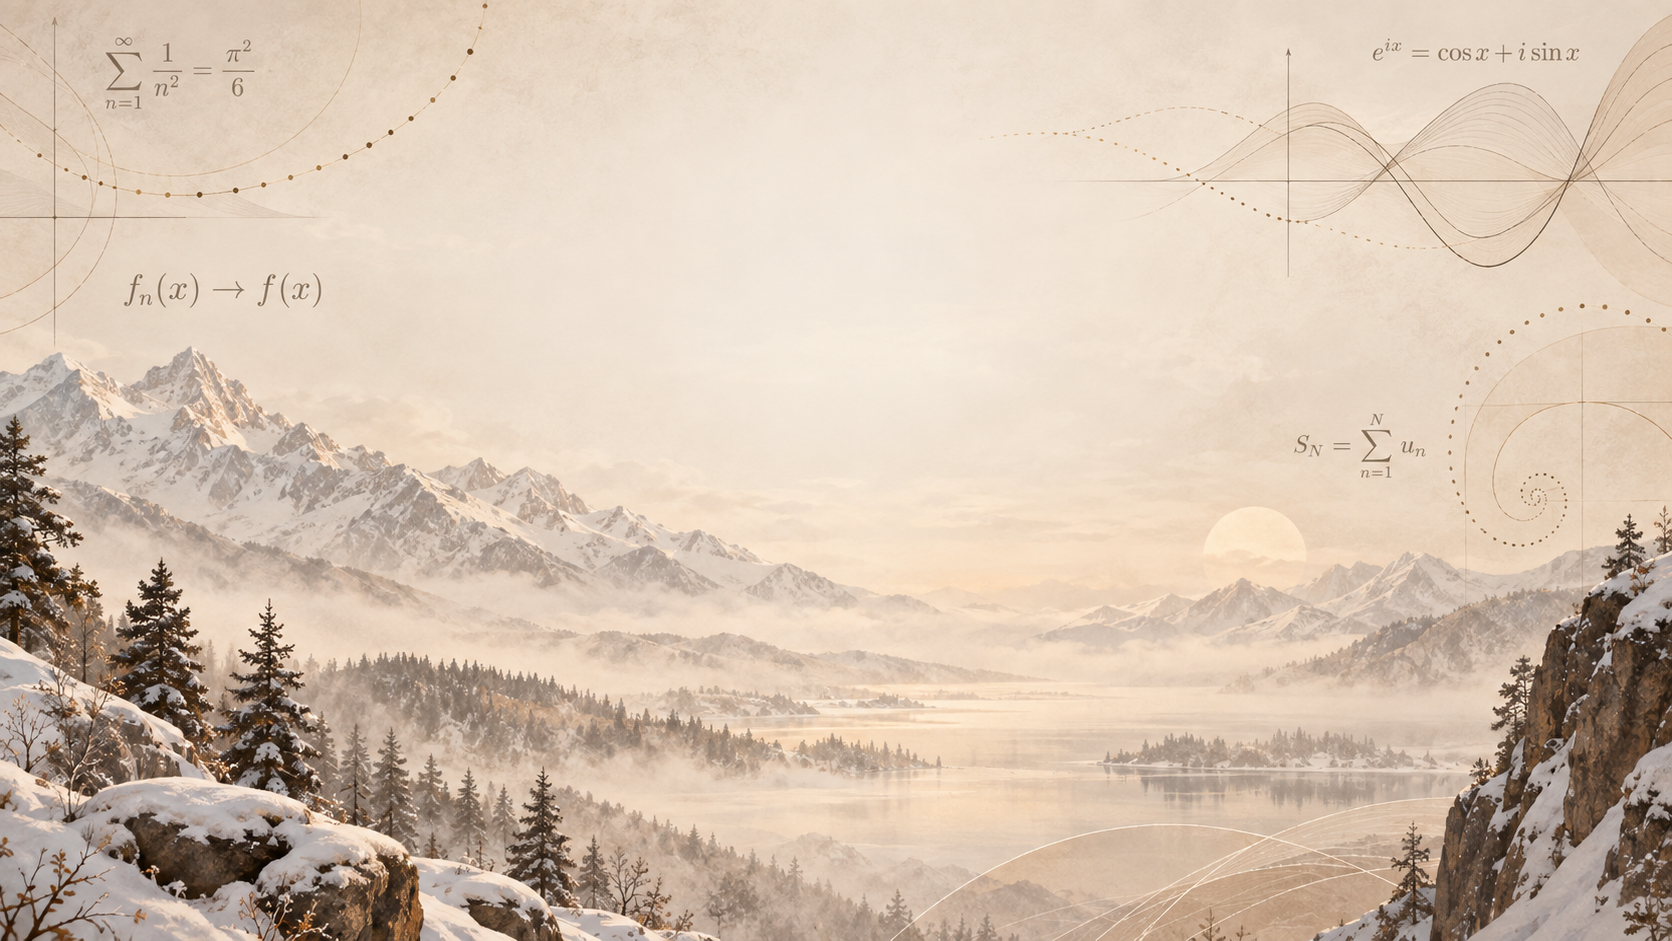
\includegraphics[width=\paperwidth,height=\paperheight,keepaspectratio=false]{chapter_07_bg_03.png}%
}
\section{Proof of Differentiating a Limit}

% --- Build 1/2 ---
\begin{frame}{Proof Strategy: Theorem 7.17}
  \begin{hlbox}
  \textbf{Part 1:} $\{f_n\}$ converges \alert{uniformly}.
  \begin{itemize}
    \item Show $\{f_n\}$ is uniformly Cauchy (Theorem 7.8)
    \item Tools: Cauchy at $x_0$ $+$ mean value theorem for $f_n - f_m$
  \end{itemize}
  \end{hlbox}

  \note{
    The proof has two parts. In Part 1 we show that the functions "f"
    sub "n" converge uniformly. As usual, we do this with the Cauchy
    criterion, Theorem 7.8, which says that a sequence converges
    uniformly if and only if it is uniformly Cauchy. The two
    ingredients are the Cauchy property of the numbers at "x" sub zero,
    and the mean value theorem applied to the difference "f" sub "n"
    minus "f" sub "m".
  }
\end{frame}

% --- Build 2/2 ---
\begin{frame}{Proof Strategy: Theorem 7.17}
  \begin{hlbox}
  \textbf{Part 1:} $\{f_n\}$ converges \alert{uniformly}.
  \begin{itemize}
    \item Show $\{f_n\}$ is uniformly Cauchy (Theorem 7.8)
    \item Tools: Cauchy at $x_0$ $+$ mean value theorem for $f_n - f_m$
  \end{itemize}

  \vspace{0.4em}
  \textbf{Part 2:} $f'(x) = \lim f_n'(x)$.
  \begin{itemize}
    \item Write derivatives as limits of \alert{difference quotients}
    \item Interchange the limits $t \to x$ and $n \to \infty$ (Theorem 7.11)
  \end{itemize}
  \end{hlbox}

  \note{
    In Part 2 we prove the formula for the derivative. A derivative is
    a limit of difference quotients, so the formula asks us to swap two
    limits: the limit as "t" approaches "x", and the limit as "n" goes
    to infinity. Theorem 7.11 from the previous section allows such a
    swap whenever one of the convergences is uniform. Our job will be
    to show that the difference quotients converge uniformly.
  }
\end{frame}

\begin{frame}{Proof of Theorem 7.17 --- Step 1: Choosing $N$}
  \begin{proofblock}{Step 1}
    Let $\varepsilon > 0$. Choose $N$ such that $n \ge N$, $m \ge N$ implies
    \begin{equation}
      |f_n(x_0) - f_m(x_0)| < \frac{\varepsilon}{2} \tag{28}
    \end{equation}
    and
    \begin{equation}
      |f'_n(t) - f'_m(t)| < \frac{\varepsilon}{2(b - a)}
      \qquad (a \leq t \leq b). \tag{29}
    \end{equation}
  \end{proofblock}

  \vspace{0.2em}
  \hl{\small (28): $\{f_n(x_0)\}$ is Cauchy. \quad
  (29): $\{f_n'\}$ is \alert{uniformly} Cauchy (Theorem 7.8).}

  \note{
    Fix a positive epsilon. We choose one index capital "N" that does two
    jobs at once. Inequality 28 says that the values at "x" sub zero are
    within epsilon over 2 of each other. Inequality 29 says that the
    derivatives are within epsilon divided by twice the length of the
    interval of each other, at every point "t" at once. The line at the
    bottom explains why both are possible: a convergent sequence of
    numbers is Cauchy, and a uniformly convergent sequence of functions is
    uniformly Cauchy, by Theorem 7.8. The odd looking denominator in 29 is
    chosen so that, after multiplying by the length of the interval, we
    get exactly epsilon over 2.
  }
\end{frame}

\begin{frame}{Proof of Theorem 7.17 --- Step 2: Mean Value Theorem}
  \begin{remblock}{Recall: Theorem 5.19 (mean value inequality)}
    $|g(x) - g(t)| \le |x - t| \cdot |g'(\xi)|$ for some $\xi$ between $x$ and $t$.
  \end{remblock}
  \begin{proofblock}{Step 2: apply it to $g = f_n - f_m$}
    By (29), for any $x, t \in [a,b]$ and $n, m \ge N$:
    \begin{equation}
      |f_n(x) - f_m(x) - f_n(t) + f_m(t)|
      \le \frac{|x - t|\,\varepsilon}{2(b - a)} \le \frac{\varepsilon}{2}. \tag{30}
    \end{equation}
  \end{proofblock}

  \note{
    The gray box recalls the mean value inequality of Theorem 5.19: the
    change of a function between two points is at most the distance
    between the points times the size of the derivative somewhere in
    between, at some point xi. This form works for complex valued functions too, which
    is why Rudin cites it here instead of the ordinary mean value
    theorem. We apply it to the difference "g" equals "f"
    sub "n" minus "f" sub "m". Its derivative is "f" sub "n" prime minus
    "f" sub "m" prime, which by 29 is smaller than epsilon divided by
    twice the length of the interval. This gives inequality 30. The middle bound will be
    reused in Part 2, and since the distance between "x" and "t" is at
    most "b" minus "a", the right side is at most epsilon over 2.
  }
\end{frame}

% --- Build 1/2 ---
\begin{frame}{Proof of Theorem 7.17 --- Step 3: Uniformly Cauchy}
  \begin{columns}[T]
    \begin{column}{0.44\textwidth}
      \begin{proofblock}{Step 3}
        With $g = f_n - f_m$:
        \[
          |g(x)| \le |g(x) - g(x_0)| + |g(x_0)|
        \]
        By (30) and (28):
        \[
          |f_n(x) - f_m(x)| < \frac{\varepsilon}{2} + \frac{\varepsilon}{2} = \varepsilon
        \]
        for all $x \in [a,b]$, $n, m \ge N$.
      \end{proofblock}
    \end{column}
    \begin{column}{0.54\textwidth}
      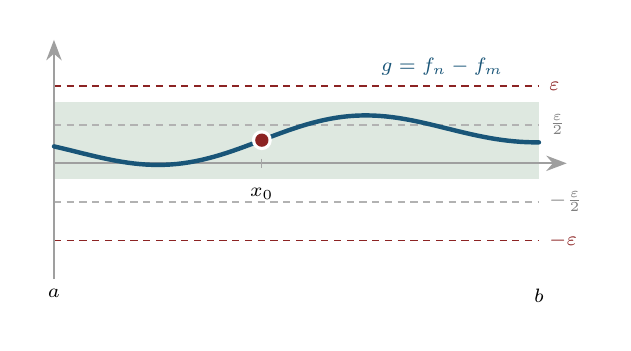
\begin{tikzpicture}[bgveil, x=0.88cm, y=0.98cm]
        \fill[proofcolor!15] (0,-0.2) rectangle (7,0.8);
        \draw[thmcolor, projln] (0,1) -- (7,1) node[right, font=\scriptsize]{$\varepsilon$};
        \draw[thmcolor, projln] (0,-1) -- (7,-1) node[right, font=\scriptsize]{$-\varepsilon$};
        \draw[gray!60, projln] (0,0.5) -- (7,0.5) node[right, font=\scriptsize, gray]{$\tfrac{\varepsilon}{2}$};
        \draw[gray!60, projln] (0,-0.5) -- (7,-0.5) node[right, font=\scriptsize, gray]{$-\tfrac{\varepsilon}{2}$};
        \draw[axisln] (0,-1.5) -- (0,1.6);
        \draw[axisln] (0,0) -- (7.4,0);
        \draw[defcolor, curveln, domain=0:7, samples=80]
          plot (\x, {0.3+0.38*sin(deg(0.9*(\x-3)))*cos(deg(0.35*(\x-3)))});
        \dotpt{thmcolor}{(3,0.3)}
        \draw[gray!70] (3,0.06) -- (3,-0.06);
        \node[below, font=\scriptsize] at (3,-0.2) {$x_0$};
        \node[below, font=\scriptsize] at (0,-1.5) {$a$};
        \node[below, font=\scriptsize] at (7,-1.5) {$b$};
        \node[defcolor, font=\scriptsize] at (5.6,1.25) {$g = f_n - f_m$};
      \end{tikzpicture}
    \end{column}
  \end{columns}

  \note{
    Now we combine the two facts. Write "g" for "f" sub "n" minus "f" sub
    "m". The triangle inequality on the slide splits "g" of "x" into two
    pieces: the change of "g" from "x" sub zero to "x", and the value at
    "x" sub zero. The picture shows "g" over the interval from "a" to "b".
    The red dot is "g" of "x" sub zero; by 28 it lies within epsilon over
    2 of zero, that is, between the gray dashed lines. By 30, the blue
    graph of "g" never moves more than epsilon over 2 away from that dot,
    so it stays inside the green strip. And however the dot and the strip
    sit, the strip always fits inside the band between the red dashed
    lines at plus and minus epsilon. Adding the two halves gives the bound
    epsilon.
  }
\end{frame}

% --- Build 2/2 ---
\begin{frame}{Proof of Theorem 7.17 --- Step 3: Uniformly Cauchy}
  \begin{columns}[T]
    \begin{column}{0.44\textwidth}
      \begin{proofblock}{Step 3}
        With $g = f_n - f_m$:
        \[
          |g(x)| \le |g(x) - g(x_0)| + |g(x_0)|
        \]
        By (30) and (28):
        \[
          |f_n(x) - f_m(x)| < \frac{\varepsilon}{2} + \frac{\varepsilon}{2} = \varepsilon
        \]
        for all $x \in [a,b]$, $n, m \ge N$.
      \end{proofblock}
    \end{column}
    \begin{column}{0.54\textwidth}
      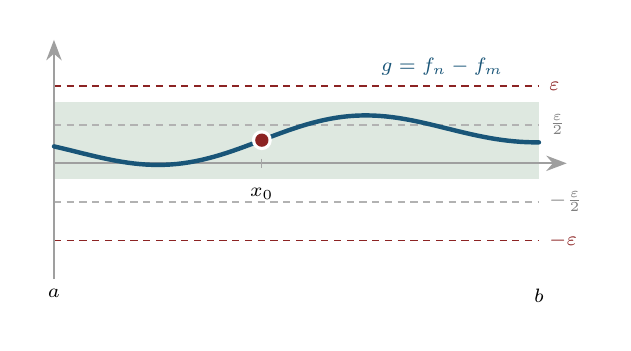
\begin{tikzpicture}[bgveil, x=0.88cm, y=0.98cm]
        \fill[proofcolor!15] (0,-0.2) rectangle (7,0.8);
        \draw[thmcolor, projln] (0,1) -- (7,1) node[right, font=\scriptsize]{$\varepsilon$};
        \draw[thmcolor, projln] (0,-1) -- (7,-1) node[right, font=\scriptsize]{$-\varepsilon$};
        \draw[gray!60, projln] (0,0.5) -- (7,0.5) node[right, font=\scriptsize, gray]{$\tfrac{\varepsilon}{2}$};
        \draw[gray!60, projln] (0,-0.5) -- (7,-0.5) node[right, font=\scriptsize, gray]{$-\tfrac{\varepsilon}{2}$};
        \draw[axisln] (0,-1.5) -- (0,1.6);
        \draw[axisln] (0,0) -- (7.4,0);
        \draw[defcolor, curveln, domain=0:7, samples=80]
          plot (\x, {0.3+0.38*sin(deg(0.9*(\x-3)))*cos(deg(0.35*(\x-3)))});
        \dotpt{thmcolor}{(3,0.3)}
        \draw[gray!70] (3,0.06) -- (3,-0.06);
        \node[below, font=\scriptsize] at (3,-0.2) {$x_0$};
        \node[below, font=\scriptsize] at (0,-1.5) {$a$};
        \node[below, font=\scriptsize] at (7,-1.5) {$b$};
        \node[defcolor, font=\scriptsize] at (5.6,1.25) {$g = f_n - f_m$};
      \end{tikzpicture}
    \end{column}
  \end{columns}

  \vspace{0.1em}
  \hl{$\Rightarrow$ $\{f_n\}$ uniformly Cauchy $\Rightarrow$ \alert{converges uniformly}
  to some $f$ (Thm.~7.8).}

  \note{
    Since this bound holds for every "x" in the interval and all "n" and
    "m" beyond capital "N", with no dependence on "x", the sequence "f"
    sub "n" is uniformly Cauchy. By Theorem 7.8 it converges uniformly to
    some function, which we call "f". This completes Part 1. Notice that
    we have not yet said anything about the derivative of "f"; we do not
    even know yet that "f" is differentiable. That is the job of Part 2.
  }
\end{frame}

\begin{frame}{Proof of Theorem 7.17 --- Part 2: Two Limits to Swap}
  \begin{columns}[T]
    \begin{column}{0.48\textwidth}
      \begin{remblock}{Recall: Theorem 7.11}
        If $\phi_n \to \phi$ \alert{uniformly} on $E$, $x$ a limit point of $E$,
        and $\lim_{t \to x} \phi_n(t) = A_n$, then $\{A_n\}$ converges and
        \[
          \lim_{t \to x} \phi(t) = \lim_{n \to \infty} A_n.
        \]
      \end{remblock}
    \end{column}
    \begin{column}{0.5\textwidth}
      \vspace{0.6em}
      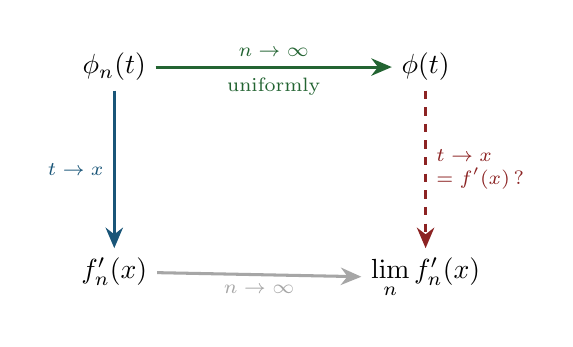
\begin{tikzpicture}[bgveil, node distance=2.0cm and 3.0cm]
        \node (tl) {$\phi_n(t)$};
        \node[right=of tl] (tr) {$\phi(t)$};
        \node[below=of tl] (bl) {$f_n'(x)$};
        \node[below=of tr] (br) {$\lim\limits_{n} f_n'(x)$};
        \draw[guide, proofcolor] (tl) -- node[above, font=\scriptsize]{$n \to \infty$}
          node[below, font=\scriptsize]{uniformly} (tr);
        \draw[guide, defcolor] (tl) -- node[left, font=\scriptsize]{$t \to x$} (bl);
        \draw[guide, gray!70] (bl) -- node[below, font=\scriptsize]{$n \to \infty$} (br);
        \draw[guide, thmcolor, dashed] (tr) -- node[right, font=\scriptsize, align=left]{$t \to x$\\ $= f'(x)$\,?} (br);
      \end{tikzpicture}
    \end{column}
  \end{columns}

  \note{
    For Part 2 we fix a point "x" and use difference quotients: phi sub
    "n" of "t" for "f" sub "n", and phi of "t" for "f". The gray box
    recalls Theorem 7.11: if functions converge uniformly and each has a
    limit at "x", then those limits converge, and the limit function has
    the corresponding limit at "x". The square on the right shows our
    plan. Going down on the left, in blue, phi sub "n" of "t" tends to "f"
    sub "n" prime of "x" as "t" approaches "x". Along the bottom, in gray,
    these derivatives converge as "n" grows, which is part of our
    hypothesis. Going right along the top, in green, we want phi sub "n"
    to converge uniformly to phi. Once we have that, Theorem 7.11 supplies
    the dashed red arrow on the right, and the limit of phi of "t" is
    exactly the derivative of "f".
  }
\end{frame}

\begin{frame}{Proof of Theorem 7.17 --- Step 4: Difference Quotients}
  \begin{columns}[T]
    \begin{column}{0.52\textwidth}
      \begin{proofblock}{Step 4}
        Fix $x \in [a,b]$. For $t \in [a,b]$, $t \ne x$:
        \begin{equation}
          \begin{gathered}
          \phi_n(t) = \frac{f_n(t) - f_n(x)}{t - x}, \\
          \phi(t) = \frac{f(t) - f(x)}{t - x}.
          \end{gathered} \tag{31}
        \end{equation}
        Then, since $f_n$ is differentiable,
        \begin{equation}
          \lim_{t \to x} \phi_n(t) = f'_n(x). \tag{32}
        \end{equation}
      \end{proofblock}
    \end{column}
    \begin{column}{0.46\textwidth}
      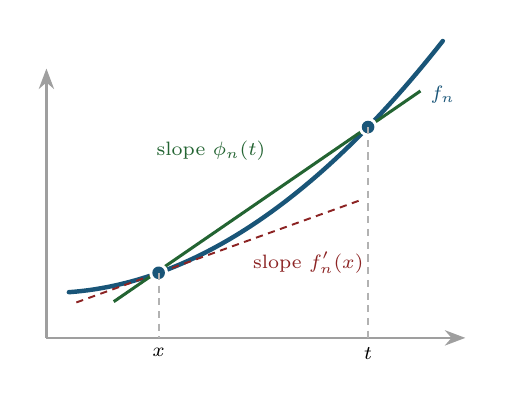
\begin{tikzpicture}[bgveil, scale=0.95]
        \draw[axisln] (0,0) -- (5.6,0);
        \draw[axisln] (0,0) -- (0,3.6);
        \draw[defcolor, curveln, domain=0.3:5.3, samples=60]
          plot (\x, {0.6+0.12*\x*\x});
        % tangent at x = 1.5: y = 0.87 + 0.36 (s - 1.5)
        \draw[thmcolor, projln] (0.4,0.474) -- (4.2,1.842);
        % secant from x=1.5 to t=4.3: y(4.3)=2.8188
        \draw[proofcolor, line width=1.1pt] (0.9,0.4842) -- (5.0,3.3008);
        \dotpt{defcolor}{(1.5,0.87)}
        \dotpt{defcolor}{(4.3,2.8188)}
        \draw[gray!60, projln] (1.5,0.87) -- (1.5,0);
        \draw[gray!60, projln] (4.3,2.8188) -- (4.3,0);
        \node[below, font=\scriptsize] at (1.5,0) {$x$};
        \node[below, font=\scriptsize] at (4.3,0) {$t$};
        \node[defcolor, font=\scriptsize] at (5.3,3.25) {$f_n$};
        \node[proofcolor, font=\scriptsize, align=center] at (2.2,2.5) {slope $\phi_n(t)$};
        \node[thmcolor, font=\scriptsize, align=center] at (3.5,1.0) {slope $f_n'(x)$};
      \end{tikzpicture}
    \end{column}
  \end{columns}

  \note{
    Here are the definitions. In equation 31, phi sub "n" of "t" is
    the difference quotient of "f" sub "n" between "x" and "t", and
    phi of "t" is the same quotient for the limit function "f". In
    the picture, the blue curve is the graph of "f" sub "n". The solid
    green line is the secant through the points above "x" and "t"; its
    slope is phi sub "n" of "t". The dashed red line is the tangent at
    "x", with slope "f" sub "n" prime of "x". Equation 32 just says that
    as "t" approaches "x", the secant slopes approach the tangent slope,
    which is the definition of the derivative.
  }
\end{frame}

% --- Build 1/2 ---
\begin{frame}{Proof of Theorem 7.17 --- Step 5: Uniform Convergence of $\phi_n$}
  \begin{proofblock}{Step 5}
    Divide the first inequality in (30) by $|x - t|$:
    \[
      |\phi_n(t) - \phi_m(t)| \le \frac{\varepsilon}{2(b - a)}
      \qquad (n \ge N,\; m \ge N),
    \]
    so $\{\phi_n\}$ is \alert{uniformly Cauchy}, hence converges uniformly,
    for $t \ne x$.
  \end{proofblock}

  \note{
    Now the key observation. The left side of inequality 30, divided by
    the distance between "x" and "t", is exactly the distance between
    phi sub "n" of "t" and phi sub "m" of "t". So the first bound in
    30 becomes the estimate on the slide, which holds for all "t"
    different from "x". The bound does not depend on "t", so the
    difference quotients are uniformly Cauchy, and hence converge
    uniformly. This is where uniform convergence of the derivatives
    pays off: through the mean value theorem, it controls every
    difference quotient at once.
  }
\end{frame}

% --- Build 2/2 ---
\begin{frame}{Proof of Theorem 7.17 --- Step 5: Uniform Convergence of $\phi_n$}
  \begin{proofblock}{Step 5}
    Divide the first inequality in (30) by $|x - t|$:
    \[
      |\phi_n(t) - \phi_m(t)| \le \frac{\varepsilon}{2(b - a)}
      \qquad (n \ge N,\; m \ge N),
    \]
    so $\{\phi_n\}$ is \alert{uniformly Cauchy}, hence converges uniformly,
    for $t \ne x$.
  \end{proofblock}
  \begin{proofblock}{Identifying the limit}
    Since $f_n \to f$, equation (31) gives
    \begin{equation}
      \lim_{n \to \infty} \phi_n(t) = \phi(t) \tag{33}
    \end{equation}
    uniformly for $a \le t \le b$, $t \ne x$.
  \end{proofblock}

  \note{
    What is the uniform limit? For each fixed "t", the numerator of
    phi sub "n" of "t" converges to "f" of "t" minus "f" of "x" by
    Part 1, while the denominator does not depend on "n". So phi sub
    "n" of "t" converges to phi of "t". Combined with the uniform
    Cauchy property, equation 33 says that the convergence is uniform.
    This is the green top arrow of our square.
  }
\end{frame}

\begin{frame}{Proof of Theorem 7.17 --- Step 6: Conclusion}
  \begin{proofblock}{Step 6: apply Theorem 7.11 to $\{\phi_n\}$}
    On $E = [a,b] \setminus \{x\}$ ($x$ is a limit point of $E$), by (32) and (33):
    \[
      \lim_{t \to x} \phi(t) = \lim_{n \to \infty} f'_n(x).
    \]
    The left side is $f'(x)$ by definition of $\phi$, so
    \[
      \boxed{\, f'(x) = \lim_{n \to \infty} f'_n(x) \,}
    \]
    which is (27). \hfill $\blacksquare$
  \end{proofblock}

  \note{
    Now we apply Theorem 7.11 on the set of all points of the interval
    except "x", which has "x" as a limit point. By 33 the difference
    quotients converge uniformly to phi, and by 32 each phi sub "n"
    has limit "f" sub "n" prime of "x" at "x". The theorem tells us that
    these limits converge, and that phi of "t" tends to their limit
    as "t" approaches "x". But the limit of phi of "t" is by
    definition the derivative of "f" at "x". So "f" is differentiable
    and equation 27 holds. The proof is complete.
  }
\end{frame}

% --- Build 1/2 ---
\begin{frame}{Remark: A Shorter Proof Under Continuity}
  \begin{remblock}{Remark}
    If, in addition, the $f'_n$ are \alert{continuous}, a much shorter proof of
    (27) can be based on Theorem 7.16 and the fundamental theorem of calculus.
  \end{remblock}

  \note{
    Rudin adds a remark. If we also assume that every derivative "f"
    sub "n" prime is continuous, there is a much shorter proof, based on
    Theorem 7.16 about integrals and the fundamental theorem of
    calculus. The extra assumption is common in practice, so this
    shortcut is worth knowing. Let's sketch it.
  }
\end{frame}

% --- Build 2/2 ---
\begin{frame}{Remark: A Shorter Proof Under Continuity}
  \begin{remblock}{Remark}
    If, in addition, the $f'_n$ are \alert{continuous}, a much shorter proof of
    (27) can be based on Theorem 7.16 and the fundamental theorem of calculus.
  \end{remblock}
  \begin{proofblock}{Sketch}
    Let $g = \lim f_n'$ (continuous by Theorem 7.12). By Theorem 6.21:
    \[
      f_n(x) = f_n(x_0) + \int_{x_0}^{x} f'_n(t)\,dt
      \;\xrightarrow[\text{Thm 7.16}]{n \to \infty}\;
      f(x) = f(x_0) + \int_{x_0}^{x} g(t)\,dt.
    \]
    By Theorem 6.20, $f' = g$ \; (as $g$ is continuous).
  \end{proofblock}

  \note{
    Call the uniform limit of the derivatives "g"; it is continuous by
    Theorem 7.12. By the fundamental theorem of calculus, Theorem 6.21,
    each "f" sub "n" at "x" equals its value at "x" sub zero plus the
    integral of its derivative from "x" sub zero to "x". Now let "n" go
    to infinity. The first term converges by hypothesis, and the
    integral converges to the integral of "g" by Theorem 7.16. So "f"
    equals a constant plus an integral of the continuous function "g",
    and by Theorem 6.20 its derivative is "g". That is equation 27.
  }
\end{frame}

% --- Build 1/2 ---
\begin{frame}{Consequence: Term-by-Term Differentiation}
  \begin{thmblock}{Corollary (series form of Theorem 7.17)}
    If each $u_k$ is differentiable on $[a,b]$, $\sum u_k(x_0)$ converges,
    and $\sum u_k'$ converges \alert{uniformly} on $[a,b]$, then
    \[
      \Bigl( \sum_{k=1}^{\infty} u_k \Bigr)' = \sum_{k=1}^{\infty} u_k'
      \qquad \text{on } [a,b].
    \]
  \end{thmblock}

  \note{
    As with continuity and integration, the theorem has a version for
    series, obtained by applying it to the partial sums. If a series of
    differentiable functions converges at one point, and the series of
    derivatives converges uniformly, then the series may be
    differentiated term by term. Rudin does not state this separately
    here, but it is how the theorem is most often used, for example for
    power series in Chapter 8.
  }
\end{frame}

% --- Build 2/2 ---
\begin{frame}{Consequence: Term-by-Term Differentiation}
  \begin{thmblock}{Corollary (series form of Theorem 7.17)}
    If each $u_k$ is differentiable on $[a,b]$, $\sum u_k(x_0)$ converges,
    and $\sum u_k'$ converges \alert{uniformly} on $[a,b]$, then
    \[
      \Bigl( \sum_{k=1}^{\infty} u_k \Bigr)' = \sum_{k=1}^{\infty} u_k'
      \qquad \text{on } [a,b].
    \]
  \end{thmblock}
  \begin{exblock}{Example}
    $\displaystyle \Bigl( \sum_{k=1}^{\infty} \frac{\sin kx}{k^3} \Bigr)'
    = \sum_{k=1}^{\infty} \frac{\cos kx}{k^2}$, \quad since
    $\Bigl| \dfrac{\cos kx}{k^2} \Bigr| \le \dfrac{1}{k^2}$ and
    $\sum \dfrac{1}{k^2} < \infty$ (M-test).
  \end{exblock}

  \note{
    Here is an example in brown. Consider the series of sine of "k" "x"
    over "k" cubed. It converges at zero, where every term vanishes. The
    differentiated series has terms cosine of "k" "x" over "k" squared,
    which are bounded by one over "k" squared, and those bounds have a
    convergent sum. So by the Weierstrass M-test, Theorem 7.10, the
    series of derivatives converges uniformly, and term by term
    differentiation is justified. Compare this with Example 7.5, where
    dividing by the square root of "n" was far too weak.
  }
\end{frame}
}

{
\usebackgroundtemplate{%
  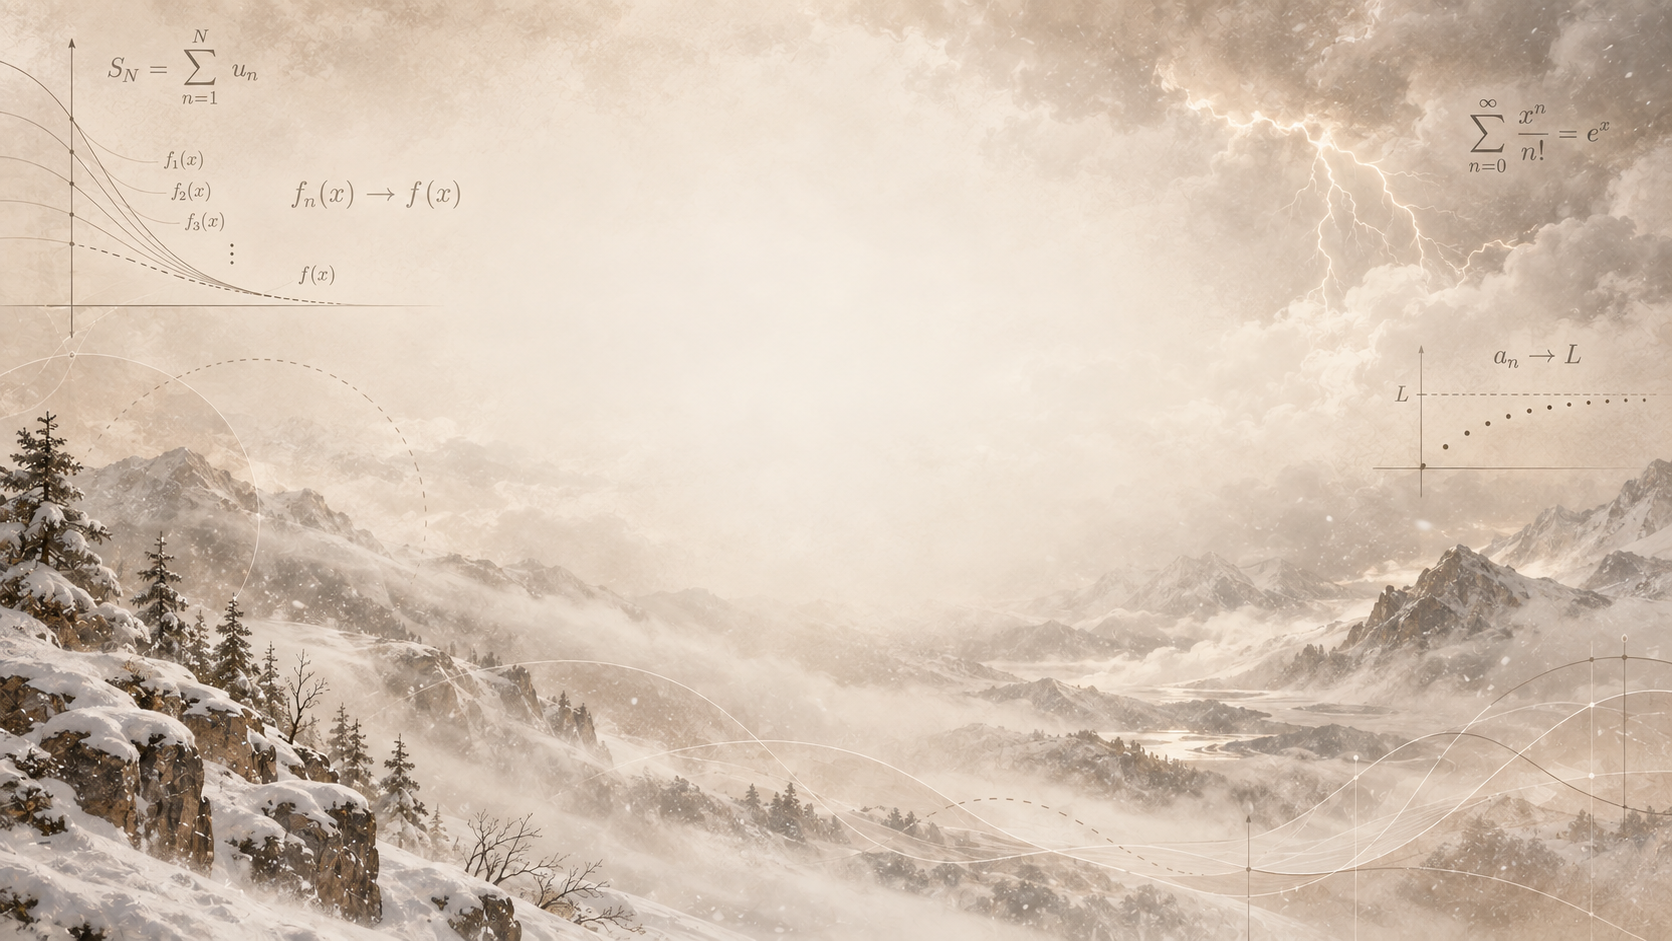
\includegraphics[width=\paperwidth,height=\paperheight,keepaspectratio=false]{chapter_07_bg_04.png}%
}
\section{Nowhere Differentiable Function}

% --- Build 1/2 ---
\begin{frame}{Theorem 7.18: A Nowhere Differentiable Function}
  \begin{thmblock}{Theorem 7.18}
    There exists a real \alert{continuous} function on the real line which is
    \alert{nowhere differentiable}.
  \end{thmblock}

  \note{
    Now we come to Theorem 7.18, one of the most surprising results in
    the book. There is a real function on the real line that is
    continuous everywhere, yet has a derivative at no point at all.
    Intuitively, a continuous function is one whose graph can be drawn
    without lifting the pen, and one tends to imagine that such a graph
    must be smooth at least somewhere. This theorem says that this
    intuition is wrong.
  }
\end{frame}

% --- Build 2/2 ---
\begin{frame}{Theorem 7.18: A Nowhere Differentiable Function}
  \begin{thmblock}{Theorem 7.18}
    There exists a real \alert{continuous} function on the real line which is
    \alert{nowhere differentiable}.
  \end{thmblock}
  \begin{remblock}{Context}
    \begin{itemize}
      \item Weierstrass (1872): $\sum a^n \cos(b^n \pi x)$ \; caused a sensation
      \item Rudin's version uses a \emph{sawtooth} instead of cosine,
        in the spirit of van der Waerden (1930)
      \item Moral: uniform limits of nice functions can be \alert{wild};
        Theorem 7.17 needs its strong hypothesis
    \end{itemize}
  \end{remblock}

  \note{
    Some context, in the gray box. The first published example was
    given by Weierstrass in 1872, as a series of cosines, and it
    shocked many mathematicians of the time. Rudin's version replaces
    the cosines by a sawtooth function, in the spirit of a simpler
    example published by van der Waerden in 1930, which makes the proof
    much shorter. For us, the moral is that a
    uniformly convergent series of continuous functions can be
    extremely rough. This explains why Theorem 7.17 needed a strong
    hypothesis on the derivatives. Let's build the example.
  }
\end{frame}

% --- Build 1/2 ---
\begin{frame}{Theorem 7.18 --- The Building Block $\varphi$}
  \begin{columns}[T]
    \begin{column}{0.47\textwidth}
      \begin{defblock}{The sawtooth}
        \begin{equation}
          \varphi(x) = |x| \quad (-1 \le x \le 1), \tag{34}
        \end{equation}
        extended to all real $x$ by
        \begin{equation}
          \varphi(x + 2) = \varphi(x). \tag{35}
        \end{equation}
      \end{defblock}
    \end{column}
    \begin{column}{0.51\textwidth}
      \begin{tikzpicture}
        \begin{axis}[
          axis background/.style={fill=white, fill opacity=0.6},
          width=8.0cm, height=3.7cm,
          xmin=-4.4, xmax=4.4, ymin=0, ymax=1.35,
          axis lines=middle, axis line style={gray!75},
          xtick={-4,-3,-2,-1,1,2,3,4}, ytick={1},
          tick label style={font=\scriptsize, fill=white, fill opacity=0.6, text opacity=1, inner sep=1pt},
          every axis plot/.append style={curveln},
        ]
          \addplot[domain=-4.3:4.3, samples=87, defcolor!45] {saw(x)};
          \addplot[domain=-1:1, samples=3, defcolor] {abs(x)};
        \end{axis}
      \end{tikzpicture}
    \end{column}
  \end{columns}

  \note{
    The construction starts with a very simple function, called phi. By
    equation 34, on the interval from minus 1 to 1 it is the absolute
    value function, which is the dark blue wedge in the middle of the
    picture. By equation 35, it repeats with period 2, giving the light
    blue sawtooth on the rest of the line, shown here from minus 4 to 4.
    So phi zigzags between 0 at the even integers and 1 at the odd
    integers, with slope plus or minus 1 on each piece. It is continuous,
    but it has a corner at every integer, which already hints at how we
    will destroy differentiability.
  }
\end{frame}

% --- Build 2/2 ---
\begin{frame}{Theorem 7.18 --- The Building Block $\varphi$}
  \begin{columns}[T]
    \begin{column}{0.47\textwidth}
      \begin{defblock}{The sawtooth}
        \begin{equation}
          \varphi(x) = |x| \quad (-1 \le x \le 1), \tag{34}
        \end{equation}
        extended to all real $x$ by
        \begin{equation}
          \varphi(x + 2) = \varphi(x). \tag{35}
        \end{equation}
      \end{defblock}
    \end{column}
    \begin{column}{0.51\textwidth}
      \begin{tikzpicture}
        \begin{axis}[
          axis background/.style={fill=white, fill opacity=0.6},
          width=8.0cm, height=3.7cm,
          xmin=-4.4, xmax=4.4, ymin=0, ymax=1.35,
          axis lines=middle, axis line style={gray!75},
          xtick={-4,-3,-2,-1,1,2,3,4}, ytick={1},
          tick label style={font=\scriptsize, fill=white, fill opacity=0.6, text opacity=1, inner sep=1pt},
          every axis plot/.append style={curveln},
        ]
          \addplot[domain=-4.3:4.3, samples=87, defcolor!45] {saw(x)};
          \addplot[domain=-1:1, samples=3, defcolor] {abs(x)};
        \end{axis}
      \end{tikzpicture}
      \begin{proofblock}{Key properties}
        For all real $s$ and $t$:
        \begin{equation}
          |\varphi(s) - \varphi(t)| \le |s - t|, \tag{36}
        \end{equation}
        $\Rightarrow$ $\varphi$ continuous on $R^1$; \; $0 \le \varphi \le 1$.
      \end{proofblock}
    \end{column}
  \end{columns}

  \note{
    Two properties of phi will be used. Inequality 36 says that phi
    never changes faster than its input: the difference of two values
    is at most the distance between the two points. This holds because
    every piece of the sawtooth has slope plus or minus 1. In
    particular phi is continuous. Also, the values of phi always lie
    between 0 and 1.
  }
\end{frame}

% --- Build 1/2 ---
\begin{frame}{Theorem 7.18 --- The Function $f$}
  \begin{columns}[T]
    \begin{column}{0.43\textwidth}
      \begin{defblock}{Definition}
        \begin{equation}
          f(x) = \sum_{n=0}^{\infty} \left(\tfrac{3}{4}\right)^n \varphi(4^n x). \tag{37}
        \end{equation}
      \end{defblock}
    \end{column}
    \begin{column}{0.55\textwidth}
      \begin{tikzpicture}
        \begin{axis}[
          axis background/.style={fill=white, fill opacity=0.6},
          width=8.6cm, height=5.0cm,
          xmin=0, xmax=2, ymin=0, ymax=3.4,
          axis lines=left, axis line style={gray!75},
          xtick={0,0.5,1,1.5,2}, ytick={0,1,2,3},
          legend pos=north west, legend cell align=left,
          legend style={font=\footnotesize, fill=white, fill opacity=0.85,
            text opacity=1, draw=gray!40, inner sep=1.5pt, row sep=-1pt},
          tick label style={font=\scriptsize, fill=white, fill opacity=0.6, text opacity=1, inner sep=1pt},
        ]
          \addplot[domain=0:2, samples=3, gray!60, line width=1.1pt] {saw(x)};
          \addplot[domain=0:2, samples=9, defcolor!70, line width=1.1pt]
            {saw(x) + 0.75*saw(4*x)};
          \addplot[domain=0:2, samples=2049, thmcolor, line width=0.8pt]
            {saw(x) + 0.75*saw(4*x) + 0.5625*saw(16*x) + 0.421875*saw(64*x)
             + 0.31640625*saw(256*x) + 0.2373046875*saw(1024*x)};
          \legend{$n = 0$, $n \le 1$, $n \le 5$}
        \end{axis}
      \end{tikzpicture}

      \begin{hlbox}
      \small
      Term $n$: height $\left(\tfrac34\right)^n$ \alert{shrinks},
      slopes $\pm 3^n$ \alert{grow}.
      \end{hlbox}
    \end{column}
  \end{columns}

  \note{
    Now we define "f" in equation 37 as a sum of scaled and compressed
    copies of phi. The term with index "n" squeezes the sawtooth
    horizontally by a factor of 4 to the power "n", and shrinks its height
    by a factor of three quarters to the power "n". As the box under the
    plot says, the heights shrink, but the slopes, which are 4 to the
    power "n" times three quarters to the power "n", equal plus or minus 3
    to the power "n" and grow. The plot shows partial sums on the interval
    from 0 to 2, as the legend in the top left corner explains: in gray just phi, labeled "n" equals 0, in blue the first
    two terms, and in red the first six terms, which is already a very
    jagged curve. The full function "f" has corners at every scale.
  }
\end{frame}

% --- Build 2/2 ---
\begin{frame}{Theorem 7.18 --- The Function $f$}
  \begin{columns}[T]
    \begin{column}{0.43\textwidth}
      \begin{defblock}{Definition}
        \begin{equation}
          f(x) = \sum_{n=0}^{\infty} \left(\tfrac{3}{4}\right)^n \varphi(4^n x). \tag{37}
        \end{equation}
      \end{defblock}

      \begin{proofblock}{$f$ is continuous}
        $0 \le \varphi \le 1$, \;$\sum (\tfrac34)^n < \infty$\\
        $\Rightarrow$ uniform (Thm.~7.10)\\
        $\Rightarrow$ continuous (Thm.~7.12)
      \end{proofblock}
    \end{column}
    \begin{column}{0.55\textwidth}
      \begin{tikzpicture}
        \begin{axis}[
          axis background/.style={fill=white, fill opacity=0.6},
          width=8.6cm, height=5.0cm,
          xmin=0, xmax=2, ymin=0, ymax=3.4,
          axis lines=left, axis line style={gray!75},
          xtick={0,0.5,1,1.5,2}, ytick={0,1,2,3},
          legend pos=north west, legend cell align=left,
          legend style={font=\footnotesize, fill=white, fill opacity=0.85,
            text opacity=1, draw=gray!40, inner sep=1.5pt, row sep=-1pt},
          tick label style={font=\scriptsize, fill=white, fill opacity=0.6, text opacity=1, inner sep=1pt},
        ]
          \addplot[domain=0:2, samples=3, gray!60, line width=1.1pt] {saw(x)};
          \addplot[domain=0:2, samples=9, defcolor!70, line width=1.1pt]
            {saw(x) + 0.75*saw(4*x)};
          \addplot[domain=0:2, samples=2049, thmcolor, line width=0.8pt]
            {saw(x) + 0.75*saw(4*x) + 0.5625*saw(16*x) + 0.421875*saw(64*x)
             + 0.31640625*saw(256*x) + 0.2373046875*saw(1024*x)};
          \legend{$n = 0$, $n \le 1$, $n \le 5$}
        \end{axis}
      \end{tikzpicture}

      \begin{hlbox}
      \small
      Term $n$: height $\left(\tfrac34\right)^n$ \alert{shrinks},
      slopes $\pm 3^n$ \alert{grow}.
      \end{hlbox}
    \end{column}
  \end{columns}

  \note{
    Why is "f" continuous? Each term is at most three quarters to the power
    "n", because phi lies between 0 and 1, and these bounds form a
    convergent geometric series. By the M-test, Theorem 7.10, the
    series converges uniformly on the whole line. Each term is
    continuous, so by Theorem 7.12 the uniform limit "f" is continuous.
    The hard part is to show that "f" has no derivative anywhere.
  }
\end{frame}
}

{
\usebackgroundtemplate{%
  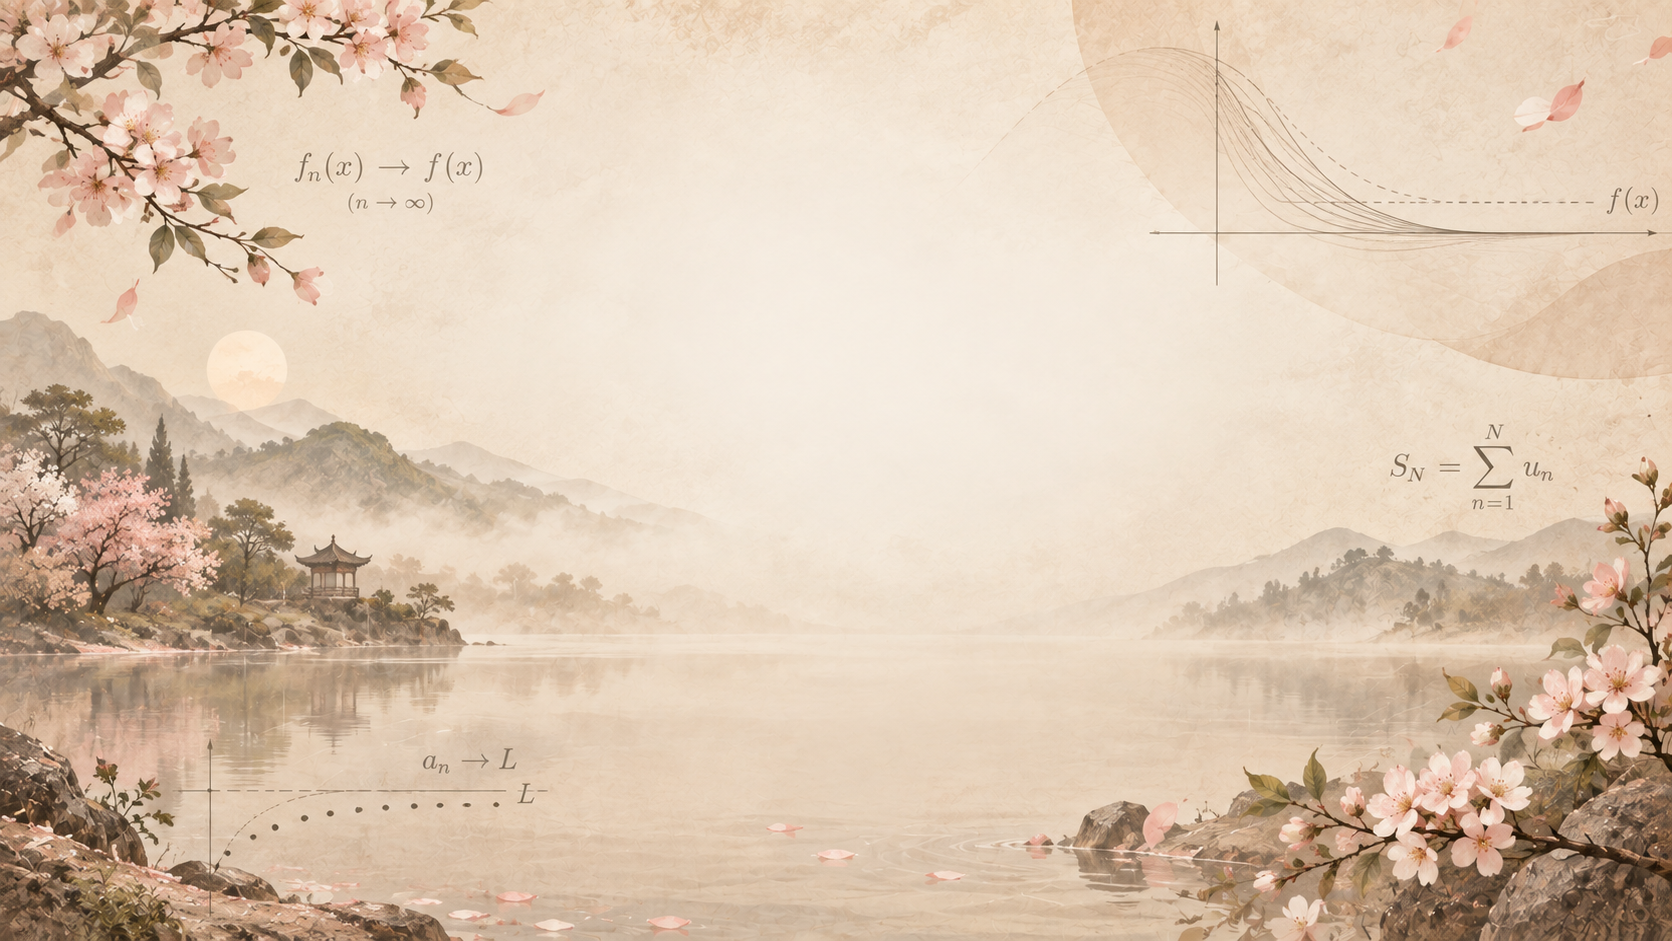
\includegraphics[width=\paperwidth,height=\paperheight,keepaspectratio=false]{chapter_07_bg_05.png}%
}
\section{Proof of Nowhere Differentiability}

% --- Build 1/3 ---
\begin{frame}{Proof Strategy: Theorem 7.18}
  \begin{hlbox}
  \textbf{Goal:} Fix any $x$. Show $f$ is \alert{not} differentiable at $x$.

  \vspace{0.6em}
  \textbf{Approach:}
  \begin{enumerate}
    \item Choose steps $\delta_m \to 0$ adapted to the term with index $m$
  \end{enumerate}
  \end{hlbox}

  \note{
    Here is the plan. We fix an arbitrary real number "x" and show that
    "f" is not differentiable there. If "f" had a derivative at "x",
    every sequence of difference quotients with steps tending to zero
    would converge to it. So it is enough to find one sequence of
    steps, delta sub "m", tending to zero, along which the difference
    quotients blow up. The first step is to choose delta sub "m" in a
    way adapted to the term with index "m" of the series.
  }
\end{frame}

% --- Build 2/3 ---
\begin{frame}{Proof Strategy: Theorem 7.18}
  \begin{hlbox}
  \textbf{Goal:} Fix any $x$. Show $f$ is \alert{not} differentiable at $x$.

  \vspace{0.6em}
  \textbf{Approach:}
  \begin{enumerate}
    \item Choose steps $\delta_m \to 0$ adapted to the term with index $m$
    \item Terms with $n > m$ \alert{vanish}; terms with $n < m$ are \emph{small}
  \end{enumerate}
  \end{hlbox}

  \note{
    With this choice, the difference quotient of "f" splits into the
    contributions of the individual terms. The terms with index larger
    than "m" contribute nothing at all, because the step lands on a
    full period of their sawtooth. The terms with index smaller than
    "m" contribute something, but we can bound it.
  }
\end{frame}

% --- Build 3/3 ---
\begin{frame}{Proof Strategy: Theorem 7.18}
  \begin{hlbox}
  \textbf{Goal:} Fix any $x$. Show $f$ is \alert{not} differentiable at $x$.

  \vspace{0.6em}
  \textbf{Approach:}
  \begin{enumerate}
    \item Choose steps $\delta_m \to 0$ adapted to the term with index $m$
    \item Terms with $n > m$ \alert{vanish}; terms with $n < m$ are \emph{small}
    \item The term $n = m$ \alert{dominates}: quotient $\ge \tfrac12(3^m + 1) \to \infty$
  \end{enumerate}
  \end{hlbox}

  \note{
    Finally, the term with index exactly "m" contributes a slope of size 3
    to the power "m", which beats the sum of all the earlier terms
    together. So the difference quotients are at least one half of the
    quantity 3 to the power "m" plus 1, which tends to infinity. A finite
    derivative is then impossible. Let's carry this out.
  }
\end{frame}

% --- Build 1/2 ---
\begin{frame}{Proof of Theorem 7.18 --- Step 1: Choosing $\delta_m$}
  \begin{proofblock}{Step 1}
    Fix $x \in R^1$ and a positive integer $m$. Put
    \begin{equation}
      \delta_m = \pm \tfrac{1}{2} \cdot 4^{-m} \tag{38}
    \end{equation}
    where the sign is chosen so that\\
    \alert{no integer} lies between $4^m x$ and $4^m(x + \delta_m)$.
  \end{proofblock}

  \note{
    We fix "x" and a positive integer "m". Equation 38 defines the step
    delta sub "m" as plus or minus one half times 4 to the power minus "m".
    The sign is the subtle part: it is chosen so that, after we multiply
    by 4 to the power "m", no integer lies strictly between the two points 4
    to the power "m" times "x" and 4 to the power "m" times "x" plus delta sub "m".
    Why can we always do this? The next build shows it.
  }
\end{frame}

% --- Build 2/2 ---
\begin{frame}{Proof of Theorem 7.18 --- Step 1: Choosing $\delta_m$}
  \begin{proofblock}{Step 1}
    Fix $x \in R^1$ and a positive integer $m$. Put
    \begin{equation}
      \delta_m = \pm \tfrac{1}{2} \cdot 4^{-m} \tag{38}
    \end{equation}
    where the sign is chosen so that\\
    \alert{no integer} lies between $4^m x$ and $4^m(x + \delta_m)$.
  \end{proofblock}

  \begin{columns}[T]
    \begin{column}{0.4\textwidth}
      \begin{hlbox}
      \small\raggedright
      Possible since $4^m |\delta_m| = \tfrac12$: one half-step from
      $y = 4^m x$ stays in the unit interval of $y$.
      \end{hlbox}
    \end{column}
    \begin{column}{0.58\textwidth}
      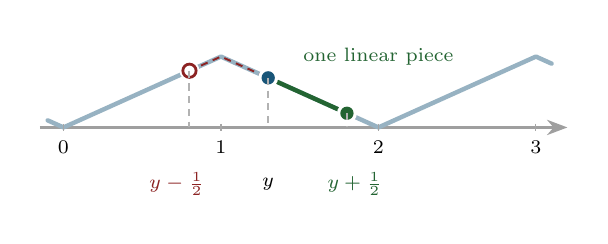
\begin{tikzpicture}[bgveil, x=2.0cm, y=0.9cm]
        \draw[axisln] (-0.15,0) -- (3.2,0);
        \draw[defcolor!45, curveln] (-0.1,0.1) -- (0,0) -- (1,1) -- (2,0) -- (3,1) -- (3.1,0.9);
        \foreach \k in {0,1,2,3} {
          \draw[gray!70] (\k,0.05) -- (\k,-0.05) node[below, font=\scriptsize, black]{$\k$};
        }
        % y = 1.3
        \draw[proofcolor, line width=1.6pt] (1.3,0.7) -- (1.8,0.2);
        \draw[thmcolor, projln] (0.8,0.8) -- (1,1) -- (1.3,0.7);
        \dotpt{defcolor}{(1.3,0.7)}
        \dotpt{proofcolor}{(1.8,0.2)}
        \opendotpt{thmcolor}{(0.8,0.8)}
        \draw[gray!60, projln] (1.3,0.7) -- (1.3,0);
        \draw[gray!60, projln] (1.8,0.2) -- (1.8,0);
        \draw[gray!60, projln] (0.8,0.8) -- (0.8,0);
        \node[font=\scriptsize] at (1.3,-0.8) {$y$};
        \node[font=\scriptsize, proofcolor] at (1.85,-0.8) {$y + \tfrac12$};
        \node[font=\scriptsize, thmcolor] at (0.72,-0.8) {$y - \tfrac12$};
        \node[font=\scriptsize, proofcolor] at (2.0,1.0) {one linear piece};
      \end{tikzpicture}
    \end{column}
  \end{columns}

  \note{
    Write "y" for 4 to the power "m" times "x". After multiplying by 4 to
    the power "m", the step becomes plus or minus one half, which is the
    point of the text on the left. In the picture, "y" is the blue point,
    lying between the integers 1 and 2 on the sawtooth. Stepping left by
    one half, to the red open point labeled "y" minus one half, would
    cross the integer 1, where the sawtooth has a corner. Stepping right,
    to the green point labeled "y" plus one half, stays inside the same
    unit interval, so the green segment lies on one linear piece. Since
    "y" is at most one half away from one end of its unit interval, one of
    the two directions always works.
  }
\end{frame}

% --- Build 1/3 ---
\begin{frame}{Proof of Theorem 7.18 --- Step 2: The Quotients $\gamma_n$}
  \begin{proofblock}{Step 2}
    Define
    \begin{equation}
      \gamma_n = \frac{\varphi(4^n(x + \delta_m)) - \varphi(4^n x)}{\delta_m}. \tag{39}
    \end{equation}
    Then, by (37),
    \(
      \dfrac{f(x + \delta_m) - f(x)}{\delta_m}
      = \displaystyle\sum_{n=0}^{\infty} \left(\tfrac34\right)^n \gamma_n.
    \)
  \end{proofblock}

  \note{
    Equation 39 defines gamma sub "n", the difference quotient of the
    sawtooth term with index "n", without its factor three quarters to the
    "n". Since "f" is a convergent sum of such terms, the difference
    quotient of "f" with step delta sub "m" is the sum of three quarters to
    the "n" times gamma sub "n", as shown on the slide. Now we examine
    the numbers gamma sub "n" in three ranges of "n".
  }
\end{frame}

% --- Build 2/3 ---
\begin{frame}{Proof of Theorem 7.18 --- Step 2: The Quotients $\gamma_n$}
  \begin{proofblock}{Step 2}
    Define
    \begin{equation}
      \gamma_n = \frac{\varphi(4^n(x + \delta_m)) - \varphi(4^n x)}{\delta_m}. \tag{39}
    \end{equation}
    Then, by (37),
    \(
      \dfrac{f(x + \delta_m) - f(x)}{\delta_m}
      = \displaystyle\sum_{n=0}^{\infty} \left(\tfrac34\right)^n \gamma_n.
    \)
  \end{proofblock}
  \begin{hlbox}
  \begin{itemize}
    \item $n > m$: \; $4^n \delta_m = \pm 2 \cdot 4^{\,n-m-1}$ is
      \alert{even} $\Rightarrow$ $\gamma_n = 0$ \; (period 2)
  \end{itemize}
  \end{hlbox}

  \note{
    First, take "n" larger than "m". Then 4 to the power "n" times delta sub
    "m" equals plus or minus 2 times a power of 4, which is an even
    integer. Since phi has period 2, shifting its argument by an even
    integer does not change its value. So the numerator of gamma sub
    "n" is zero, and gamma sub "n" is zero. All the terms beyond index
    "m" drop out, and the infinite sum becomes a finite one.
  }
\end{frame}

% --- Build 3/3 ---
\begin{frame}{Proof of Theorem 7.18 --- Step 2: The Quotients $\gamma_n$}
  \begin{proofblock}{Step 2}
    Define
    \begin{equation}
      \gamma_n = \frac{\varphi(4^n(x + \delta_m)) - \varphi(4^n x)}{\delta_m}. \tag{39}
    \end{equation}
    Then, by (37),
    \(
      \dfrac{f(x + \delta_m) - f(x)}{\delta_m}
      = \displaystyle\sum_{n=0}^{\infty} \left(\tfrac34\right)^n \gamma_n.
    \)
  \end{proofblock}
  \begin{hlbox}
  \begin{itemize}
    \item $n > m$: \; $4^n \delta_m = \pm 2 \cdot 4^{\,n-m-1}$ is
      \alert{even} $\Rightarrow$ $\gamma_n = 0$ \; (period 2)
    \item $0 \le n \le m$: \; by (36), $|\gamma_n| \le 4^n |\delta_m| / |\delta_m| = 4^n$
    \item $n = m$: \; $|\gamma_m| = 4^m$ \; (slope $\pm 1$ on one piece, Step 1)
  \end{itemize}
  \end{hlbox}

  \note{
    Next, for "n" between zero and "m", inequality 36 bounds the
    numerator by 4 to the power "n" times the size of delta sub "m", so the
    size of gamma sub "n" is at most 4 to the power "n". Finally, for "n"
    equal to "m" this bound is attained exactly. By the choice of the
    sign in Step 1, the two points 4 to the power "m" times "x" and 4 to the
    "m" times "x" plus delta sub "m" lie on one straight piece of the
    sawtooth, where the slope is plus or minus 1. So the size of gamma
    sub "m" is exactly 4 to the power "m".
  }
\end{frame}

% --- Build 1/2 ---
\begin{frame}{Proof of Theorem 7.18 --- Step 3: The Estimate}
  \begin{proofblock}{Step 3}
    \vspace{-0.6em}
    \begin{align*}
      \left|\frac{f(x + \delta_m) - f(x)}{\delta_m}\right|
      &= \left|\sum_{n=0}^{m} \left(\tfrac{3}{4}\right)^n \gamma_n\right|
      \;\ge\; \underbrace{\left(\tfrac34\right)^m 4^m}_{\text{term } n = m}
        - \sum_{n=0}^{m-1} \left(\tfrac34\right)^n 4^n \\
      &= 3^m - \sum_{n=0}^{m-1} 3^n
      \;=\; 3^m - \frac{3^m - 1}{2}
      \;=\; \boxed{\tfrac{1}{2}(3^m + 1)}.
    \end{align*}
  \end{proofblock}

  \note{
    Now we put the pieces together. Since the terms beyond "m" vanish,
    the difference quotient is a finite sum up to "m". By the reverse
    triangle inequality, its size is at least the size of the last
    term minus the sizes of all the others. The last term is three quarters
    to the power "m" times 4 to the power "m", which is 3 to the power "m". The earlier
    terms are at most 3 to the power "n" each, and their geometric sum is 3 to
    the "m" minus 1, over 2. Subtracting gives the boxed bound, one half
    of the quantity 3 to the power "m" plus 1. The dominant term wins by a factor of about
    two.
  }
\end{frame}

% --- Build 2/2 ---
\begin{frame}{Proof of Theorem 7.18 --- Step 3: The Estimate}
  \begin{proofblock}{Step 3}
    \vspace{-0.6em}
    \begin{align*}
      \left|\frac{f(x + \delta_m) - f(x)}{\delta_m}\right|
      &= \left|\sum_{n=0}^{m} \left(\tfrac{3}{4}\right)^n \gamma_n\right|
      \;\ge\; \underbrace{\left(\tfrac34\right)^m 4^m}_{\text{term } n = m}
        - \sum_{n=0}^{m-1} \left(\tfrac34\right)^n 4^n \\
      &= 3^m - \sum_{n=0}^{m-1} 3^n
      \;=\; 3^m - \frac{3^m - 1}{2}
      \;=\; \boxed{\tfrac{1}{2}(3^m + 1)}.
    \end{align*}
  \end{proofblock}
  \begin{proofblock}{Conclusion}
    As $m \to \infty$: \; $\delta_m \to 0$, but the quotients $\to \infty$.\\
    Hence $f$ is \alert{not differentiable at $x$}. Since $x$ was arbitrary,
    $f$ is nowhere differentiable. \hfill $\blacksquare$
  \end{proofblock}

  \note{
    As "m" goes to infinity, the steps delta sub "m" tend to zero, while
    the difference quotients are at least one half of the quantity 3 to
    the power "m" plus 1, which tends to infinity. If "f" were
    differentiable at "x", these quotients would have to converge to the
    finite number "f" prime of "x". So "f" is not differentiable at "x".
    Since "x" was an arbitrary real number, "f" is differentiable nowhere,
    and the proof is complete.
  }
\end{frame}

% --- Build 1/3 ---
\begin{frame}{Why the Construction Works}
  \begin{remblock}{The balance of $\tfrac34$ and $4$}
    \begin{itemize}
      \item Heights $\left(\tfrac34\right)^n$: summable $\Rightarrow$ $f$ is
        \alert{continuous}
    \end{itemize}
  \end{remblock}

  \note{
    Let's step back and see why the construction works. The gray box
    lists the competing effects. The first is the heights: three quarters
    to the power "n" form a convergent geometric series. That is all we
    needed for uniform convergence, and hence for continuity of "f".
    The sawtooth terms get smaller fast enough that adding them up
    never tears the graph apart.
  }
\end{frame}

% --- Build 2/3 ---
\begin{frame}{Why the Construction Works}
  \begin{remblock}{The balance of $\tfrac34$ and $4$}
    \begin{itemize}
      \item Heights $\left(\tfrac34\right)^n$: summable $\Rightarrow$ $f$ is
        \alert{continuous}
      \item Slopes $\left(\tfrac34 \cdot 4\right)^n = 3^n$: each one exceeds the
        \emph{sum} of all earlier ones $\Rightarrow$ \alert{no derivative}
    \end{itemize}
  \end{remblock}

  \note{
    The second effect is the slopes. Each term has slope plus or minus
    3 to the power "n", and 3 to the power "m" is larger than the sum of all the
    earlier slopes, which is 3 to the power "m" minus 1, over 2. So the newest
    and finest wiggle always dominates the difference quotient, no
    matter how small the step. Heights shrink, slopes explode: this
    mismatch is the whole secret.
  }
\end{frame}

% --- Build 3/3 ---
\begin{frame}{Why the Construction Works}
  \begin{remblock}{The balance of $\tfrac34$ and $4$}
    \begin{itemize}
      \item Heights $\left(\tfrac34\right)^n$: summable $\Rightarrow$ $f$ is
        \alert{continuous}
      \item Slopes $\left(\tfrac34 \cdot 4\right)^n = 3^n$: each one exceeds the
        \emph{sum} of all earlier ones $\Rightarrow$ \alert{no derivative}
      \item Same proof for $\sum a^n \varphi(b^n x)$ with $0 < a < 1$,
        $4 \mid b$, $ab > 2$:\\
        quotients $\ge (ab)^m \dfrac{ab - 2}{ab - 1} \to \infty$
    \end{itemize}
  \end{remblock}

  \note{
    Nothing is special about three quarters and 4. The same proof works for
    the series with coefficients "a" to the power "n" and frequencies "b" to
    the "n", as long as "a" is between 0 and 1, "b" is a multiple of 4,
    and the product "a" "b" exceeds 2; the vertical bar on the slide
    means that 4 divides "b". The multiple of 4 makes the
    later terms vanish, exactly as in Step 2, and the condition on the
    product makes the dominant term win, giving the lower bound on the
    slide, which tends to infinity. This is the same balance as in
    Weierstrass's original cosine example.
  }
\end{frame}
}

{
\usebackgroundtemplate{%
  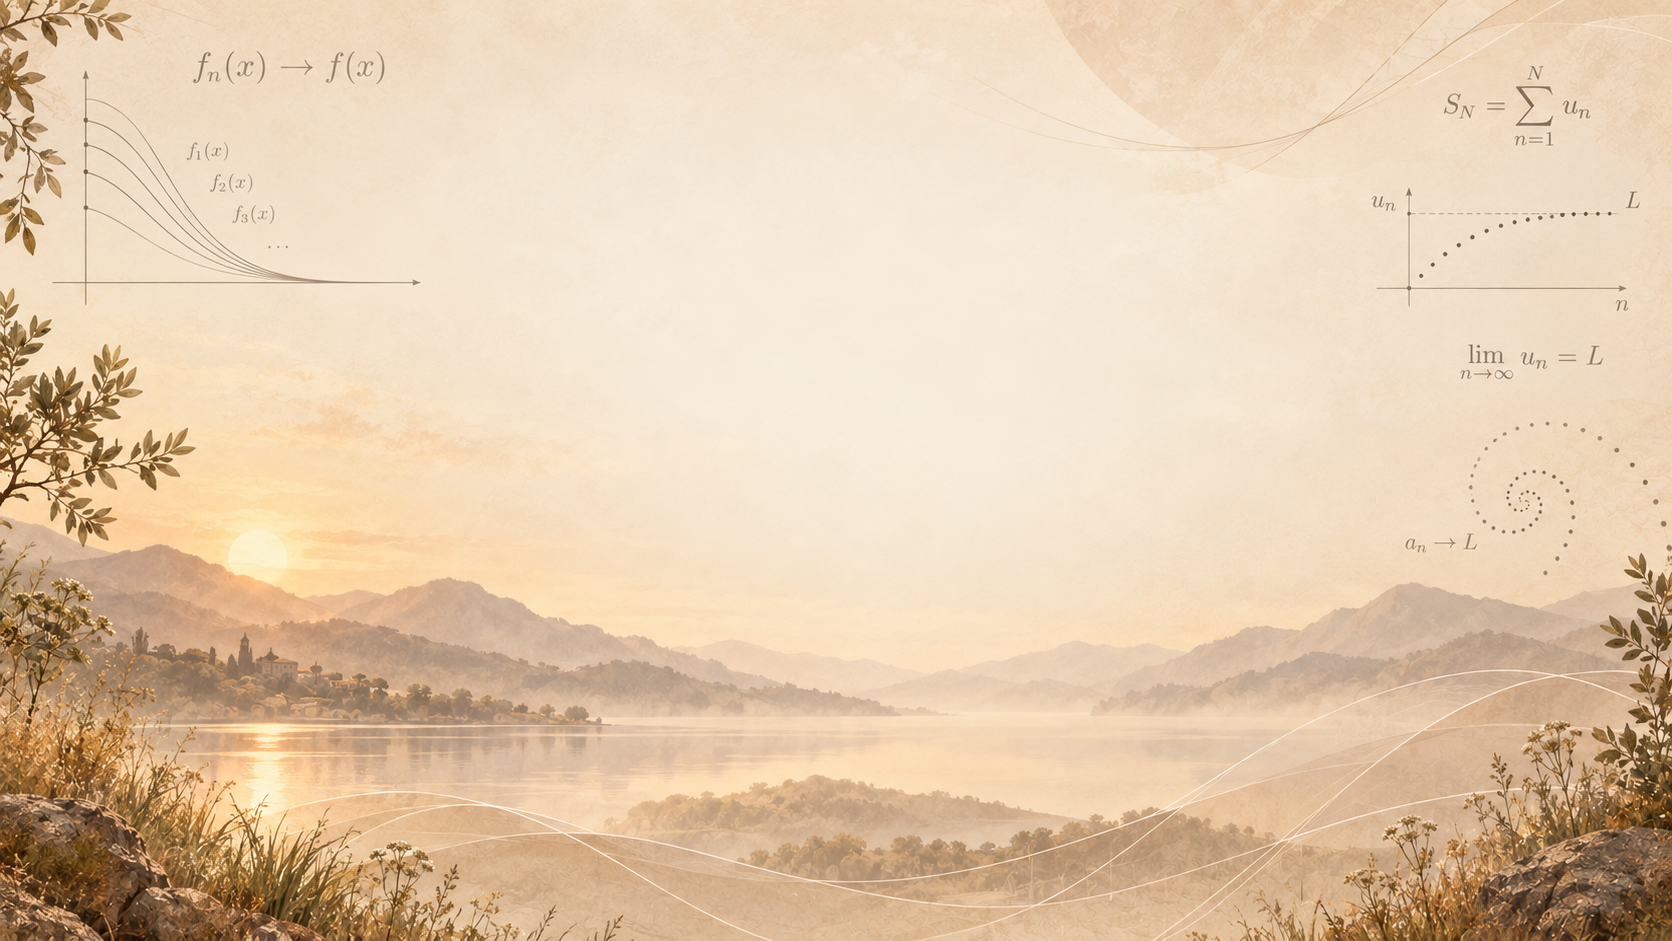
\includegraphics[width=\paperwidth,height=\paperheight,keepaspectratio=false]{chapter_07_bg_06.png}%
}
\section{Summary}

% --- Build 1/3 ---
\begin{frame}{Summary}
  \begin{hlbox}
  \textbf{Key takeaways from this section:}
  \begin{itemize}
    \item Uniform convergence of $f_n$ says \alert{nothing} about $f_n'$
      (Example 7.5)
  \end{itemize}
  \end{hlbox}

  \note{
    Let's review. We began with the observation from Example 7.5 that
    uniform convergence of the functions gives no control over their
    derivatives, because small values can hide large slopes. The
    functions sine of "n" "x" over the square root of "n" shrink to zero
    uniformly, while their slopes grow without bound.
  }
\end{frame}

% --- Build 2/3 ---
\begin{frame}{Summary}
  \begin{hlbox}
  \textbf{Key takeaways from this section:}
  \begin{itemize}
    \item Uniform convergence of $f_n$ says \alert{nothing} about $f_n'$
      (Example 7.5)
    \item \textbf{Theorem 7.17:} $f_n(x_0)$ converges and $f_n' \to$
      \alert{uniformly} on $[a,b]$\\
      $\Rightarrow$ $f_n \to f$ uniformly and $f' = \lim f_n'$
    \item \textbf{Proof:} mean value theorem $+$ Theorem 7.11
  \end{itemize}
  \end{hlbox}

  \note{
    Theorem 7.17 gives the right hypothesis: convergence at a single
    point, plus uniform convergence of the derivatives. Then the
    functions converge uniformly, and the derivative of the limit is the
    limit of the derivatives. The proof used the mean value theorem to
    turn control of slopes into control of values and of difference
    quotients, and then Theorem 7.11 to swap the two limits.
  }
\end{frame}

% --- Build 3/3 ---
\begin{frame}{Summary}
  \begin{hlbox}
  \textbf{Key takeaways from this section:}
  \begin{itemize}
    \item Uniform convergence of $f_n$ says \alert{nothing} about $f_n'$
      (Example 7.5)
    \item \textbf{Theorem 7.17:} $f_n(x_0)$ converges and $f_n' \to$
      \alert{uniformly} on $[a,b]$\\
      $\Rightarrow$ $f_n \to f$ uniformly and $f' = \lim f_n'$
    \item \textbf{Proof:} mean value theorem $+$ Theorem 7.11
    \item \textbf{Theorem 7.18:} $\sum (\tfrac34)^n \varphi(4^n x)$ is
      continuous but \alert{nowhere differentiable}
  \end{itemize}

  \vspace{0.4em}
  \textbf{Coming up next:} equicontinuous families of functions.
  \end{hlbox}

  \note{
    Theorem 7.18 showed how wild a uniform limit can be: a series of
    shrinking, compressed sawtooth functions converges uniformly to a
    continuous function with no derivative anywhere. In the next
    section, Equicontinuous Families of Functions, we ask a different
    question: when does a sequence of functions have a uniformly
    convergent subsequence? The answer leads to the Arzela Ascoli
    theorem. See you next time.
  }
\end{frame}
}

\end{document}
